% =====================================================================
%  Rosetta — prétirage arXiv (version française)
%  Compilation :  pdflatex rosetta-fr && bibtex rosetta-fr &&
%                 pdflatex rosetta-fr && pdflatex rosetta-fr
%
%  Traduction de ../en/rosetta.tex. La structure, les étiquettes (\label), les
%  références et la bibliographie sont identiques à la version anglaise, de
%  sorte que les deux fichiers restent comparables ligne à ligne section par
%  section. Le CODE des listings est laissé tel quel, commentaires compris :
%  c'est du code, et l'environnement lstlisting ne tolère pas les caractères
%  accentués sous inputenc/T1.
% =====================================================================
\documentclass[11pt,a4paper]{article}

\usepackage[utf8]{inputenc}
\usepackage[T1]{fontenc}
\usepackage[french]{babel}
\usepackage{lmodern}
\usepackage{microtype}
\usepackage[margin=2.6cm]{geometry}
\usepackage{amsmath,amssymb}
\usepackage{booktabs}
\usepackage{longtable}
\usepackage{graphicx}
\usepackage{listings}
\usepackage{xcolor}
\usepackage{tikz}
\usetikzlibrary{arrows.meta,positioning,fit,backgrounds}
\usepackage[hidelinks]{hyperref}

% --- aides à la rédaction ------------------------------------------
\newcommand{\todo}[1]{\textcolor{red}{\textbf{[À FAIRE : #1]}}}
\newcommand{\gap}[1]{\textcolor{orange}{\textsf{\small$\langle$#1$\rangle$}}}

% --- listings ------------------------------------------------------
\definecolor{codebg}{gray}{0.96}
\lstdefinestyle{cpp}{
  language=C++, basicstyle=\ttfamily\footnotesize,
  keywordstyle=\color{blue!60!black}, commentstyle=\color{gray},
  stringstyle=\color{green!40!black},
  backgroundcolor=\color{codebg}, frame=none,
  showstringspaces=false, breaklines=true, columns=fullflexible,
  morekeywords={consteval,constexpr,requires,concept,template,auto,co_await}
}
\lstset{style=cpp}

% --- abréviations --------------------------------------------------
\newcommand{\rosetta}{\textsc{Rosetta}}
\newcommand{\code}[1]{\texttt{\small #1}}

% =====================================================================
\title{\textbf{La réflexion comme langage de description d'interfaces :\\
projections statiques et dynamiques d'API C++ vers plusieurs langages}}

\author{
  Frantz Maerten\\
  \small\itshape{Look Up Geoscience}\\
  \small\itshape{Géosciences Montpellier}\\
  \small\texttt{fmaerten@gmail.com}
  % \and
  % Bruno L\'evy\\
  % Inria Nancy\\
  % \small\texttt{Bruno.Levy@inria.fr}
}

\date{\today}

\begin{document}
\maketitle

% =====================================================================
\begin{abstract}
Exposer une bibliothèque C++ à un autre langage se fait normalement une fois par
cible : un module \code{pybind11/nanobind} écrit à la main pour Python, une couche N-API
pour Node, un usertype \code{sol2} pour Lua, une couche de transfert pour C\#,
et une hiérarchie de classes annotées pour moc dans une interface Qt. Chacune de
ces couches redit, d'une manière différente, une information que le compilateur C++ possède déjà.

Nous présentons \rosetta, un système qui lit cette information une seule fois
--- par la réflexion statique de C++26 (P2996) sur des en-têtes
\emph{non modifiés} --- pour la placer dans une représentation intermédiaire
(RI) indépendante de la cible, puis qui \emph{projette} cette représentation de
deux façons. La projection \emph{statique} produit du code C++ ordinaire pour
dix-neuf cibles ; pour dix-sept d'entre elles, le code produit ne contient
aucune réflexion et se compile avec n'importe quel compilateur C++20,
plutôt qu'avec la branche expérimentale que la réflexion exige elle-même. La
projection \emph{dynamique} écrit la même information sous forme de tables de
métadonnées statiques, ce qui donne un modèle méta-objet accessible à
l'exécution, que scripts et interfaces graphiques interrogent par nom sans avoir
été compilés contre les en-têtes de la bibliothèque.

L'observation centrale est qu'il ne s'agit pas de deux fonctionnalités mais d'un
seul mécanisme vu de deux côtés, ne différant que par le \emph{moment} où les
noms sont résolus. Nous le démontrons par une conséquence mesurable : cinq
cibles dont la surface de liaison est indexée par nom --- Lua, Node,
WebAssembly, C\# et Java --- doivent abandonner les ensembles de surcharges C++
au moment de la génération, et pourtant les retrouvent intégralement par la
projection dynamique, parce que la résolution passe du temps de génération au
temps d'appel. La différence d'expressivité entre cibles n'est donc pas une
propriété du langage cible, mais de son moment de résolution.

\rosetta{} traite en outre la couverture de liaison comme un artefact de premier
plan : tout membre non exposé est consigné, avec une raison exploitable par
outil, dans un \code{coverage.json} que l'on peut comparer d'une révision à
l'autre. Sur une API contrôlée de 288 méthodes, les cinq cibles indexées par nom
en lient 96 quel que soit le nombre de surcharges déclarées, tandis que la
projection à liaison tardive les atteint toutes les 288 --- deux tiers de
l'interface récupérés par le seul report de la résolution. Pointé sur une
bibliothèque de maillages tierce non modifiée et chargé de lier l'intégralité de
son espace de noms public sans assistance, le pipeline atteint 75\,\% de ce
qu'on lui donne, et la raison de l'échec du reste est concentrée plutôt que
diffuse : un quart de la surface déclarée de cette bibliothèque est constitué de
patrons, et 85\,\% de ceux-ci se trouvent dans ses types-valeurs vecteur et
matrice plutôt que dans les algorithmes qu'un appelant invoque.
\end{abstract}

\noindent\textbf{Mots-clés :} réflexion statique, C++26, liaisons de langages,
représentation intermédiaire, protocole méta-objet, logiciel scientifique.

% =====================================================================
\section{Introduction}
\label{sec:intro}

Une bibliothèque scientifique C++ reste rarement en C++. Ses utilisateurs la
veulent depuis Python pour l'analyse, depuis Julia pour le calcul numérique,
depuis un carnet de notes, depuis un navigateur, derrière un point d'accès REST,
et depuis une interface graphique qui leur permet de déplacer un curseur et de
voir un résultat. Chacun de ces usages est aujourd'hui un projet d'ingénierie
distinct, avec ses idiomes, ses modes de défaillance et sa charge de maintenance
propres --- et chacun commence par redire des faits que le compilateur C++
connaît déjà parfaitement : que \code{Mesh} possède un champ nommé
\code{opacity} de type \code{double}, que \code{at} est surchargée sur
\code{int} et sur \code{int,int}, que \code{Solver} dérive de \code{Operator}.

Cette redite est le coût dont traite cet article. Il est payé $N$ fois pour $N$
cibles, il dérive silencieusement lorsque l'API C++ évolue, et il explique
pourquoi tant de bibliothèques scientifiques n'ont exactement qu'une liaison ---
Python, en général --- et aucune voie crédible vers une deuxième.

La réflexion statique de C++26~\cite{p2996} change ce qui est possible ici, car
pour la première fois l'information est disponible \emph{depuis l'intérieur du
langage}, avec les réponses du compilateur lui-même aux questions qu'un
analyseur tiers doit reconstituer : quelle surcharge est masquée par une
déclaration dérivée, quels membres spéciaux sont implicitement déclarés, quelle
base est publique, comment s'écrit réellement une spécialisation de patron. Un
système bâti là-dessus n'a pas besoin d'embarquer son propre frontal C++.

Mais la réflexion seule ne produit pas de liaisons, et la traiter comme un
meilleur analyseur syntaxique, c'est la sous-employer. Cet article défend une
position plus forte :

\begin{quote}\itshape
La réflexion statique peut servir de mécanisme de description d'interfaces
indépendant du langage. Un seul parcours réflexif d'une bibliothèque C++ non
modifiée fournit une représentation intermédiaire dont on peut projeter
\emph{à la fois} des liaisons statiques sans réflexion \emph{et} un modèle
méta-objet persistant à l'exécution --- les deux projections ne différant que
par le moment où la résolution des noms a lieu.
\end{quote}

\paragraph{Contributions.}
\begin{enumerate}
  \item \textbf{Une RI indépendante de la cible, dérivée de la réflexion.} Un
    unique parcours \code{consteval} d'un type transmet chaque membre, avec son
    lot complet d'annotations, à un visiteur. Les moteurs de génération ne
    voient jamais \code{std::meta::info} (section~\ref{sec:ir}).
  \item \textbf{Une projection statique vers dix-neuf cibles hétérogènes} ---
    liaisons de langages, documentation, schémas et interfaces utilisateur ---
    à partir de cette unique description (section~\ref{sec:static}).
  \item \textbf{Un déploiement sans réflexion.} La réflexion est confinée à
    l'étape de génération : pour dix-sept des dix-neuf cibles, le code produit
    n'exige que C++20 et se compile donc avec n'importe quel compilateur publié
    plutôt qu'avec la branche expérimentale dont la réflexion a elle-même besoin
    (section~\ref{sec:pipeline}). Les deux exceptions sont délibérées et
    exposées à la section~\ref{sec:limitations}.
  \item \textbf{Une projection dynamique} : la même RI écrite sous forme de
    tables de métadonnées statiques, donnant un modèle méta-objet interrogeable
    par nom à l'exécution par un script ou une interface graphique, sans
    connaître les types C++ (section~\ref{sec:dynamic}).
  \item \textbf{Le moment de résolution comme axe structurant.} Nous montrons
    que l'expressivité perdue par les cibles à liaison précoce est récupérée par
    la projection à liaison tardive, et nous la quantifions
    (section~\ref{sec:resolution}).
  \item \textbf{La couverture comme artefact de premier plan, lisible par
    outil} : ce qui n'a pas été lié, et pourquoi (section~\ref{sec:coverage}).
\end{enumerate}

\paragraph{Ce que nous ne prétendons pas.}
Nous ne prétendons pas que \rosetta{} produit de meilleures liaisons Python
qu'un module \code{pybind11} ou \code{nanobind} écrit à la main ; un expert disposant d'un temps
illimité l'emportera toujours sur une cible donnée. Nous affirmons que c'est le
coût \emph{par cible} que \rosetta{} supprime. Nous ne prétendons pas davantage
que le modèle méta-objet soit en lui-même nouveau --- le système méta-objet de
Qt~\cite{qt}, le GOM de Graphite~\cite{graphite}, la réflexion UObject
d'Unreal~\cite{unreal} et Objective-C le précèdent tous de loin. La nouveauté
est
que le modèle est \emph{dérivé automatiquement, par le compilateur, à partir
d'en-têtes non modifiés}, et qu'il partage sa description avec les liaisons
statiques.

% =====================================================================
\section{Motivation : le coût par cible}
\label{sec:motivation}

\subsection{Une méthode, cinq notations}

Considérons une unique fonction membre d'une petite classe numérique --- un
tampon plat de scalaires groupés en éléments :

\begin{lstlisting}[caption={La déclaration. Tout ce qui suit en est dérivé.},label={lst:decl}]
namespace serie {
    class Serie {
    public:
        std::size_t itemSize() const;   // scalars per item
        // ...
    };
}
\end{lstlisting}

Le listing~\ref{lst:five} montre ce que coûte l'exposition de cette seule
fonction dans cinq environnements hôtes. Chaque ligne est reprise telle quelle
de la sortie de \rosetta, mais rien n'y est propre à \rosetta{} --- c'est ce
qu'un développeur écrit à la main, et ce que contient le module manuscrit
correspondant.

\begin{lstlisting}[caption={La même fonction membre, cinq fois.},label={lst:five}]
// pybind11
c.def("itemSize", &serie::Serie::itemSize, "Scalars per item: ...");

// N-API (Node)
props.push_back(This::InstanceMethod<&This::call_method<
                    &serie::Serie::itemSize>>("itemSize"));

// embind (WebAssembly)
.function("itemSize", static_cast<unsigned long (serie::Serie::*)() const>(
                          &serie::Serie::itemSize))

// jlcxx (Julia)
c.method("itemSize", static_cast<unsigned long (serie::Serie::*)() const>(
                         &serie::Serie::itemSize));

// sol2 (Lua)
c["itemSize"] = &serie::Serie::itemSize;
\end{lstlisting}

Cinq notations, et chacune encode les trois mêmes faits : \emph{quelle entité
C++} est exposée, \emph{quel nom} elle prend dans le langage hôte, et ---
explicitement dans les cas embind et jlcxx, implicitement dans les autres ---
\emph{quelle est sa signature}. Ces trois faits sont déjà connus du compilateur
qui vient d'analyser le listing~\ref{lst:decl}. Aucun n'est une décision de
conception ; ce sont des transcriptions.

Les deux lignes portant un \code{static\_cast} explicite méritent attention, car
elles montrent la transcription échouer d'une manière facile à manquer :
\code{\&Serie::itemSize} désigne un \emph{ensemble de surcharges}, non une
fonction, si bien qu'une cible incapable d'accepter un ensemble de surcharges
doit épeler la signature pour en choisir un membre. Cette écriture doit ensuite
suivre la déclaration à la main. C'est exactement le genre de fait dupliqué qui
dérive.

\subsection{Le coût est différentiel, pas seulement initial}

Écrire cinq liaisons une fois est une dépense bornée, quoique fastidieuse. La
dépense récurrente, c'est que l'API C++ bouge. Une méthode ajoutée à
\code{Serie} doit être ajoutée cinq fois de plus, dans cinq notations, dans cinq
fichiers ; un paramètre renommé, un type de retour modifié ou une nouvelle
surcharge se propagent de la même façon.

Nous le mesurons à la section~\ref{sec:e2} : sur trois cibles, le code de
liaison qu'un humain écrirait croît de 67 lignes par classe, et quatre fichiers
source générés changent à \emph{chaque} montée de version de la bibliothèque.
Rien dans cette arithmétique ne dépend du fait que les liaisons soient
générées --- 67 lignes par classe, c'est ce qu'un développeur maintiendrait
autrement.

Pire, le mode de défaillance est silencieux. Une méthode que personne n'a pensé
à ajouter au module Lua est indiscernable, vue de l'extérieur, d'une méthode qui
n'avait jamais vocation à s'y trouver : le module ne l'a tout simplement pas, et
aucune étape de compilation ne proteste. C'est cette observation qui motive de
faire de la couverture de liaison un artefact explicite et lisible par outil,
plutôt qu'une déduction à partir de ce qui compile
(section~\ref{sec:coverage}).

\subsection{Le problème du second ordre : des interfaces sur les mêmes faits}

Une liaison n'est pas le seul consommateur de la structure d'un type. Un panneau
de propriétés doit savoir que \code{Serie} possède un \code{itemSize}, de quel
type il est, s'il est modifiable et quelle plage il peut prendre. Un inspecteur
en console, une vue QML, une surcouche de débogage en mode immédiat et un schéma
REST ont tous besoin de la même chose. Chacun est une redite supplémentaire des
mêmes faits et, comme chacun vise une boîte à outils différente, chacun est
écrit séparément.

Ce n'est pas hypothétique : c'est à quoi ressemblait le dépôt de \rosetta{}
lui-même. Avant l'existence de la projection dynamique, cinq parcoureurs C++
écrits à la main traversaient les mêmes métadonnées, un par consommateur --- un
interpréteur en console (446 lignes), un panneau de propriétés Qt (401), une
fenêtre principale Qt (235), un environnement d'exécution ImGui (331) et un
objet réfléchi QML (102) : environ 1\,500 lignes exprimant une seule idée cinq
fois, chacune devant être revue dès que les métadonnées changeaient de forme.

La mesure de ce qui, là-dedans, était accidentel plutôt qu'essentiel : les 401
lignes de C++ du panneau de propriétés Qt deviennent 30 lignes de Python dès que
les métadonnées sont atteignables depuis le langage hôte
(section~\ref{sec:dynamic}). Ce que faisaient surtout les parcoureurs C++,
ce n'était pas construire des widgets --- c'était re-dériver une structure que
quelque chose d'autre connaissait déjà.

\subsection{L'exigence}

Les deux problèmes ont la même forme. L'information est disponible exactement une
fois, dans le compilateur, au moment où il analyse l'en-tête ; puis elle est
ressaisie à la main, une fois par consommateur, dans la notation que ce
consommateur emploie. D'où :

\begin{quote}\itshape
La description devrait être extraite une seule fois, par l'entité qui la détient
déjà, sous une forme qui ne privilégie la notation d'aucun consommateur --- puis
projetée, autant de fois qu'il y a de consommateurs.
\end{quote}

La réflexion statique rend l'extraction possible. Le reste de cet article traite
de ce que la forme intermédiaire doit consigner pour que les projections soient
fidèles, et de ce qui arrive quand les consommateurs ne s'accordent pas sur ce
qu'ils savent exprimer.

% =====================================================================
\section{Contexte : la réflexion statique de C++26, et ce qu'elle impose}
\label{sec:background}

P2996~\cite{p2996} introduit \code{std::meta::info}, une valeur de réflexion
désignant une entité du programme, ainsi que des requêtes \code{consteval} sur
cette valeur (\code{members\_of}, \code{type\_of}, \code{identifier\_of},
\dots) et le \emph{splicing}, qui reconvertit une valeur de réflexion en
déclaration utilisable.

Deux propriétés comptent pour la suite.

\paragraph{Les réponses du compilateur, pas celles d'un analyseur.}
Comme les requêtes s'exécutent au sein d'une véritable compilation des en-têtes
de l'utilisateur, elles rapportent ce que le langage a effectivement décidé. Le
listing~\ref{lst:hiding} en est le cas canonique : \code{Derived::f(double)}
masque les deux surcharges de la base, et un appelant C++ dépourvu d'un
\code{using Base::f;} ne peut pas les atteindre. \rosetta{} lie exactement
\code{f(double)}, et consigne les deux déclarations masquées comme abandons. Un
système bâti sur un analyseur C++ indépendant doit réimplémenter le masquage de
noms, le contrôle d'accès, la déclaration implicite des membres spéciaux et
l'instanciation des patrons --- et divergera du compilateur dans les recoins.

\begin{lstlisting}[caption={Le masquage de noms est une décision du compilateur, pas une affaire de syntaxe.},label={lst:hiding}]
struct Base    { int f(int) const; int f(int, int) const; };
struct Derived : Base { int f(double) const; };
// Derived binds only f(double); the two Base overloads are recorded
// as `hidden_by_derived` drops.
\end{lstlisting}

\paragraph{La contrainte qui façonne tout le reste.}
La réflexion répond aux questions \emph{au moment de la compilation d'un
programme qui inclut les en-têtes de l'utilisateur}. Elle ne peut être
interrogée depuis un script, un système de compilation ou un fichier de
configuration. Par conséquent, pour connaître la forme d'un type, quelque chose
doit \emph{compiler} ; et pour écrire les réponses sur disque, ce quelque chose
doit \emph{s'exécuter}. Compiler-puis-exécuter n'est pas un choix
d'implémentation --- c'est la seule forme que cela puisse prendre, et c'est
pourquoi \rosetta{} est un pipeline plutôt qu'une commande. La
section~\ref{sec:pipeline} rend ce pipeline explicite.

\paragraph{Disponibilité.} P2996 est implémenté dans \code{clang-p2996}, une
branche de recherche. La section~\ref{sec:limitations} précise où cette
dépendance pèse et où elle ne pèse pas.

% =====================================================================
\section{Architecture : un pipeline à deux étapes}
\label{sec:pipeline}

\begin{figure}[t]
\centering
\begin{tikzpicture}[
  node distance=6mm,
  box/.style={draw, rounded corners=2pt, align=center, font=\small,
              minimum height=7mm, inner xsep=3mm},
  refl/.style={box, fill=blue!8},
  noreflect/.style={box, fill=green!8},
  arr/.style={-{Latex[length=2mm]}}
]
\node[box] (man) {\code{manifest.json}};
\node[box, below=of man] (gen) {\code{rosetta\_gen}\\[-1mm]{\tiny C++17 --- un gabarit JSON vers C++}};
\node[refl, below=of gen] (drv) {pilote généré, compilé par \code{clang-p2996}\\[-1mm]{\tiny \textbf{la seule étape réflexive}}};
\node[box, below=of drv, fill=yellow!12] (ir) {\textbf{RI Rosetta}\\[-1mm]{\tiny \code{GenClass} / \code{GenMethod}}\\[-1mm]{\tiny \code{GenType} / \code{GenEnum}}};

\node[noreflect, below left=10mm and 8mm of ir] (stat) {projection statique\\[-1mm]{\tiny 19 cibles, C++ produit}};
\node[noreflect, below right=10mm and 8mm of ir] (dyn) {projection dynamique\\[-1mm]{\tiny tables en \code{.rodata}}};

\node[box, below=8mm of stat] (langs) {Python, Node, Julia,\\ Lua, WASM, Qt, \dots};
\node[box, below=8mm of dyn] (mop) {\code{rosetta::script}\\[-1mm]{\tiny protocole méta-objet}};

\draw[arr] (man) -- (gen);
\draw[arr] (gen) -- (drv);
\draw[arr] (drv) -- node[right,font=\tiny] {la réflexion a lieu ici} (ir);
\draw[arr] (ir) -- (stat);
\draw[arr] (ir) -- (dyn);
\draw[arr] (stat) -- (langs);
\draw[arr] (dyn) -- (mop);

\begin{scope}[on background layer]
  \node[draw, dashed, rounded corners, fit=(stat)(dyn)(langs)(mop),
        label={[font=\tiny\itshape]below:tout ce qui est sous la RI est du C++20 ordinaire}] {};
\end{scope}
\end{tikzpicture}
\caption{Le pipeline. La réflexion n'intervient qu'en un seul endroit. La RI est
le pivot : à sa gauche la projection statique, à sa droite la projection
dynamique. Rien qui relève de la réflexion ne survit dans les artefacts
produits.}
\label{fig:pipeline}
\end{figure}

\paragraph{Étape 0 --- le gabarit.}
\code{rosetta\_gen} lit un \code{manifest.json} et produit un programme pilote
C++, un en-tête qui inclut les types de l'utilisateur, et un
\code{CMakeLists.txt}. Il n'effectue aucune réflexion et se compile avec
n'importe quel compilateur C++17 ; il n'ouvre jamais les en-têtes de
l'utilisateur, il ne fait que recopier leurs noms dans le pilote qu'il écrit. Sa
raison d'être est que ce qu'écrit l'auteur d'un projet soit un \emph{manifeste},
et non un programme.

\paragraph{Étape 1 --- réfléchir et produire.}
Le pilote est compilé avec \code{clang-p2996} puis exécuté. Pendant sa
compilation, le parcours réflexif s'exécute ; pendant son exécution, il écrit
des fichiers. C'est la séquence compiler-puis-exécuter dont la
section~\ref{sec:background} a montré qu'elle est incontournable.

\paragraph{Étapes 2--3 --- compiler et charger.}
Les projets produits sont du C++20 ordinaire. Ils sont configurés et compilés
avec un compilateur publié, puis chargés par leurs environnements hôtes. Chaque
étape a donc une exigence de langage différente et décroissante : C++17 pour
compiler le gabarit, C++26 pour exécuter le pilote réflexif, C++20 pour compiler
ce qu'il a produit.

\paragraph{La bibliothèque est lue deux fois.}
Le tableau~\ref{tab:twice} énonce la propriété qui rend possible un déploiement
sans réflexion : la première passe \emph{décrit} les types et exige C++26 ; la
seconde les \emph{appelle} et ne l'exige pas.

\begin{table}[h]
\centering\small
\begin{tabular}{llll}
\toprule
passe & par & objet & langage requis \\
\midrule
étape 1 & le pilote de réflexion & \textbf{décrire} les types & C++26 \\
étape 3 & la liaison générée & les \textbf{appeler} & C++20 \\
\bottomrule
\end{tabular}
\caption{Pourquoi les artefacts produits survivent à la chaîne d'outils de
recherche. L'exigence \emph{baisse} entre les deux passes, et c'est tout
l'intérêt : la chaîne de recherche est nécessaire pour apprendre la forme d'un
type, pas pour s'en servir.}
\label{tab:twice}
\end{table}

Il en découle une conséquence pratique qu'il vaut mieux énoncer tôt, car c'est
aussi une limitation : des annotations écrites \emph{en ligne} dans un en-tête
utilisateur y attirent \code{<experimental/meta>}, de sorte que la seconde passe
exigerait elle aussi la chaîne C++26, et la propriété d'absence de réflexion est
perdue. \rosetta{} accepte donc des annotations \emph{hors ligne} dans un
fichier JSON annexe, qui laissent les en-têtes de l'utilisateur en C++ ordinaire.
Ce mécanisme n'est pas un agrément ; c'est ce qui fait tenir l'affirmation
d'absence de réflexion pour les bibliothèques annotées
(section~\ref{sec:limitations}).

% =====================================================================
\section{La représentation intermédiaire dérivée de la réflexion}
\label{sec:ir}

\subsection{Un parcours, plusieurs visiteurs}

La surface réflexive de \rosetta{} est un unique parcours \code{consteval}. Un
visiteur implémente quatre patrons membres \code{consteval} :

\begin{lstlisting}[caption={Le concept de visiteur au complet. \code{Fld}/\code{Fn} sont des paramètres de patron non-type \code{std::meta::info} ; \code{Anns...} est le lot complet d'annotations du membre.},label={lst:walk}]
v.template field          <Fld,  Anns...>(name);
v.template method_instance<Fn,   Anns...>(name);
v.template method_static  <Fn,   Anns...>(name);
v.template constructor    <Ctor, Anns...>();   // optional, detected by requires
\end{lstlisting}

Deux décisions de conception du listing~\ref{lst:walk} portent l'essentiel de
l'architecture.

D'abord, \textbf{le parcoureur n'a pas de point d'entrée par annotation}. Il
transmet le lot d'annotations complet et laisse le visiteur décider de ce qui
l'intéresse ; un moteur qui comprend \code{range} et un moteur qui l'ignore ont
la même forme. Ajouter un type d'annotation ne touche donc pas au parcoureur.

Ensuite, et c'est plus important, \textbf{les moteurs de génération ne voient pas
la réflexion}. Au moment où un moteur s'exécute, il manipule des structures
ordinaires --- \code{GenClass}, \code{GenMethod}, \code{GenField},
\code{GenType}, \code{GenEnum} --- dont les membres sont des
\code{std::string}. L'auteur d'un moteur n'écrit aucun code \code{consteval} et
ne touche jamais à \code{std::meta::info}. C'est ce qui rend dix-neuf moteurs
gérables, et c'est la raison pour laquelle la projection dynamique est possible :
une RI faite de données ordinaires peut être écrite sur disque, ce que des
valeurs de réflexion ne peuvent pas.

\subsection{Ce que la RI consigne}

Un arbre syntaxique consigne ce que la source \emph{dit} ; une représentation
intermédiaire consigne ce qu'elle \emph{signifie}, sous une forme choisie pour
ses consommateurs plutôt que pour son producteur. Au-delà de l'évidence (noms,
types, paramètres, types de retour, bases, ensembles de surcharges,
annotations), deux catégories d'enregistrement méritent d'être isolées, car
c'est exactement là que cette distinction se joue.

\paragraph{L'identité est dédoublée.} Chaque classe porte à la fois une écriture
C++ pleinement qualifiée et un nom \emph{exposé}. La première est ce que le C++
produit doit écrire pour résoudre l'entité, classes englobantes comprises autant
qu'espaces de noms ; le second est ce que voit le langage cible, et peut être
renommé pour éviter une collision entre deux classes partageant un nom non
qualifié. C'est de les tenir séparés qui permet à une description unique de
servir des langages aux règles de nommage incompatibles.

\paragraph{Des propriétés sémantiques, non de la syntaxe.} La RI consigne si une
classe est abstraite, constructible par défaut, publiquement destructible,
assignable par copie ou déplacement et constructible par copie ou déplacement.
Cela ne se lit pas dans le texte source --- ce sont des conclusions du
compilateur --- et chacune existe parce qu'un moteur en a besoin pour éviter de
produire du code qui ne compile pas. Une classe à comptage de références dotée
d'un destructeur protégé, par exemple, est une erreur de compilation franche au
sein de tout environnement d'exécution qui détruit ce qu'il enveloppe.

\paragraph{Et ce qui a été perdu.} Chaque classe porte les membres que le
parcours n'a pu confier à aucun moteur, avec une raison : \code{no\_identifier}
(les opérateurs et les fonctions de conversion n'ont pas de nom liable),
\code{function\_template} (aucun lot de paramètres fixe à insérer) et
\code{hidden\_by\_derived}. Ces informations alimentent la
section~\ref{sec:coverage}.

% =====================================================================
\section{La projection statique}
\label{sec:static}

\subsection{Dix-neuf cibles, une description}

\begin{table}[h]
\centering\small
\begin{tabular}{ll}
\toprule
catégorie & cibles \\
\midrule
script / machine virtuelle & \code{python} (pybind11), \code{nanobind}, \code{lua} (sol2), \code{node} (N-API), \code{julia} (jlcxx) \\
web & \code{wasm} (embind), \code{typescript}, \code{rest}, \code{openapi} \\
managé & \code{csharp}, \code{java} \\
interface utilisateur & \code{qt}, \code{qml}, \code{imgui}, \code{paraview} \\
description & \code{markdown}, \code{html}, \code{json} \\
exécution & \code{dynamic} (section~\ref{sec:dynamic}) \\
\bottomrule
\end{tabular}
\caption{Les dix-neuf moteurs de génération. Leur hétérogénéité --- un module
Python, une table de routes REST, un schéma OpenAPI et une ligne de widget Qt ne
sont pas des variations sur un même thème --- est la preuve que la RI est
réellement indépendante de la cible.}
\label{tab:backends}
\end{table}

Le nombre en lui-même n'est pas une contribution ; c'est une preuve. Ce qui
compte, c'est que des cibles de \emph{catégories} différentes consomment la même
RI : un moteur REST transforme une méthode en route URL, un moteur Qt transforme
un champ en ligne de widget avec un curseur dont les bornes viennent d'une
annotation \code{range}, et un moteur Markdown transforme une classe en
documentation --- sans que rien d'autre que la RI ne leur soit commun.

\subsection{L'idiome, plutôt que la translittération mécanique}
\label{sec:idiom}

Une question de conception revient sans cesse : un type C++ doit-il traverser la
frontière tel quel, ou sous la forme de son équivalent dans le langage cible ?
La position de \rosetta{} est la seconde, partout où la cible possède un
équivalent : une séquence devrait parvenir à l'hôte comme la séquence propre à
cet hôte. \code{std::vector<double>} est une \code{list} Python et --- c'est le
sujet de cette section --- un \code{Array} JavaScript. Jusqu'où chaque cible va
dépend de ce que permet sa bibliothèque de liaison : sol2 et jlcxx exposent les
conteneurs C++ sous forme d'userdata, aussi le moteur Lua ajoute-t-il une
seconde surcharge acceptant une table à côté de celle qui prend le conteneur,
plutôt que de la remplacer. L'intérêt d'énoncer cela comme une position et non
comme un détail d'implémentation, c'est que la lecture immédiate de chaque
bibliothèque de liaison pousse dans l'autre sens, et que c'est sur la cible
WebAssembly que cette pression est la plus forte.

\paragraph{Ce que la bibliothèque propose.} embind ne donne à
\code{std::vector<T>} aucune conversion par défaut ; le remède documenté est
\code{register\_vector<T>}, qui en fait une \emph{classe liée}. Les conséquences
sont visibles à chaque ligne du code appelant : JavaScript doit construire un
\code{M.vector\_double} et le remplir par \code{push\_back}, ne peut pas passer
un littéral de tableau, reçoit une poignée plutôt qu'un \code{Array} en retour,
et doit appeler \code{.delete()} sur cette poignée. Le
listing~\ref{lst:idiom} oppose les deux formes pour les mêmes déclarations
C++ --- la \code{Serie} du listing~\ref{lst:decl}, dont le constructeur prend un
\code{std::vector<double>} et dont \code{scalars()} renvoie un
\code{const std::vector<double>\&}.

\begin{lstlisting}[language=Java,caption={Les deux mêmes signatures C++, vues depuis JavaScript. En haut : ce que donne \code{register\_vector}. En bas : ce que produit \rosetta.},label={lst:idiom}]
// with register_vector<double> - a sequence as an opaque bound class
const buf = new M.vector_double();
for (const x of [1.0, 2.0, 4.0]) buf.push_back(x);
const s0 = new M.Serie(buf, 1);
buf.delete();
const out = s0.scalars();            // an M.vector_double handle
console.log(out.get(1)); out.delete();

// what rosetta emits - the sequence is the host language's own Array
const s = new M.Serie([1.0, 2.0, 4.0], 1);
console.log(s.scalars()[1]);        // a JS Array
\end{lstlisting}

La forme du haut n'est pas fautive, et une liaison écrite à la main s'en
contenterait raisonnablement. C'était toutefois le seul endroit de \rosetta{} où
une séquence n'était pas le type tableau propre au langage hôte --- une rupture
d'idiome que l'utilisateur rencontre dès sa première ligne de code, et qu'aucune
autre cible n'imposait.

\paragraph{Ce qu'il faut pour la refermer.} Le correctif tient en une unique
spécialisation du \code{BindingType} propre à embind pour
\code{std::vector<T>}, qui le place sur le canal \code{emval} --- la technique
même que \code{<emscripten/val.h>} emploie déjà pour \code{std::optional}. En
sortie, \code{val::array(v)}, qui recopie par memcpy à travers une vue de
tableau typé lorsque \code{T} est arithmétique et parcourt élément par élément
sinon ; en entrée, \code{vecFromJSArray<T>}. Un
\code{register\_type<\dots>()} par type d'élément déclare ensuite cet
identifiant de type comme un passe-plat \code{emval} côté JavaScript ; sans
cela, le module s'interrompt au premier appel sur
\code{BindingError: Unbound type}.

Deux propriétés justifient de faire cela dans un générateur plutôt qu'à la main.
D'abord, cela se compose avec la bibliothèque au lieu de la contourner : les
relais \code{BindingType<const T>} et \code{BindingType<T\&>} propres à embind
portent l'unique spécialisation jusqu'aux paramètres et retours
\code{const std::vector<T>\&}, de sorte qu'un pointeur de fonction membre
ordinaire se lie encore --- il n'y a aucun adaptateur par méthode à produire ---
et les \code{vector<vector<T>>} imbriqués s'en déduisent par récurrence.
Ensuite, cela s'écrit une fois et vaut pour toute classe que porte la RI. La RI
dit quels membres manipulent des séquences et quels sont leurs types d'élément ;
le moteur décide, une fois, ce qu'\emph{est} une séquence en JavaScript. Cette
asymétrie --- une décision, toutes les classes --- est le levier qu'achète la
RI, et c'est le même levier ailleurs : \code{std::filesystem::path} transmis
comme une chaîne, ou un paramètre de sortie rejoignant la valeur de retour ---
un tuple en Python, des retours multiples en Lua, un tableau en JavaScript.

\paragraph{La preuve.} \code{examples/plain-binding} pilote une même classe C++
depuis quatre hôtes, avec un script pilote chacun. Après la modification, le
pilote WebAssembly est le pilote Node ligne pour ligne, aux deux seules choses
qu'embind fait véritablement autrement près --- le module se charge de façon
asynchrone et distribue des poignées d'objets que l'appelant doit
\code{.delete()} ; et un \code{throw} C++ arrive sous la forme d'une
\code{CppException} emscripten plutôt que d'une \code{TypeError}. Les séquences
ne figurent plus parmi les différences, et les deux exécutions affichent les
mêmes valeurs, à cette unique ligne d'exception près. Ce résidu est la mesure
honnête de la position : ce qui reste est ce que la cible impose réellement, et
non ce que sa bibliothèque de liaison a trouvé commode.

L'alignement sur l'idiome n'est ni gratuit ni universel. Il se paie par moteur
et par famille de types, dans du code de moteur qui doit bien connaître la
bibliothèque cible --- et il s'arrête là où la cible ne peut pas suivre. Un
\code{std::vector<T*>} ne traverse toujours pas ce canal, car \code{val::array}
exigerait une politique \code{allow\_raw\_pointers} par élément en sortie et
\code{vecFromJSArray} de même en entrée, ce que le point d'accroche
\code{BindingType} ne sait porter ni dans un sens ni dans l'autre. Un tel membre
est écarté avec une raison consignée plutôt que mal traduit
(section~\ref{sec:coverage}).

\subsection{Là où les cibles divergent : les surcharges}
\label{sec:overloads}

L'endroit où les cibles divergent le plus nettement est la surcharge C++, et il
vaut la peine de l'examiner car la section~\ref{sec:resolution} en fait un
résultat.

\begin{table}[h]
\centering\small
\begin{tabular}{lll}
\toprule
cible & politique & pourquoi \\
\midrule
\code{python} (pybind11) & toutes surcharges & des \code{.def} répétés forment un ensemble de surcharges \\
\code{nanobind}         & toutes surcharges & même modèle \\
\code{julia} (jlcxx)    & toutes surcharges & la répartition multiple choisit \\
\code{qt}               & toutes surcharges & une ligne de widget par méthode ; rien n'est indexé par nom \\
\midrule
\code{wasm} (embind)    & la première seule & un second \code{.function} lève à l'initialisation du module \\
\code{node} (N-API)     & la première seule & les descripteurs de propriété sont indexés par nom \\
\code{lua} (sol2)       & la première seule & \code{c["at"] = \dots} est une affectation \\
\code{csharp}, \code{java} & la première seule & table d'opérations indexée par nom ; transfert JSON \\
\code{typescript}       & la première seule & décrit le module N-API ; ne doit pas trop promettre \\
\code{rest}             & la première seule & une route est un chemin d'URL \\
\code{qml}              & la première seule & \code{registerInvoker} est indexé par nom \\
\bottomrule
\end{tabular}
\caption{Politique de surcharge par cible. Le clivage ne tient pas à la
puissance du langage --- Lua et JavaScript savent exprimer une répartition ---
mais à ce que la \emph{surface de liaison} soit ou non une table indexée par
nom. \og Première \fg{} signifie première déclarée, ce qui reste stable d'une
régénération à l'autre.}
\label{tab:overloads}
\end{table}

Point capital : la RI ne prend pas cette décision. Elle porte l'ensemble de
surcharges complet, et chaque moteur le réduit s'il le doit, en consignant
chaque frère écarté comme une entrée
\code{overload\_not\_expressible} du rapport de couverture. Une réduction est une
politique de moteur, jamais une perte de la RI --- ce qui est précisément
pourquoi la section~\ref{sec:resolution} peut la récupérer.

% =====================================================================
\section{La projection dynamique : un modèle méta-objet à l'exécution}
\label{sec:dynamic}

\subsection{Dépenser la RI en données plutôt qu'en code}

Tous les moteurs de la section~\ref{sec:static} dépensent le résultat de la
réflexion en \emph{appels de bibliothèque de liaison}. L'information est
consommée au moment de la génération, et ce qui en subsiste est du code pour une
seule exécution particulière.

Le moteur \code{dynamic}, lui, la dépense en \textbf{données}. Il réécrit la RI
sous forme de tables statiques --- \code{MetaClass}, \code{MetaField},
\code{MetaMethod}, \code{MetaCtor}, \code{TypeDesc}, \code{MetaEnum},
\code{MetaFunction} --- de sorte que la question \og que contient cette classe ? \fg{}
reste posable à l'exécution, par un appelant qui n'a jamais été compilé contre
les en-têtes de la bibliothèque. Les tables résident dans le \code{.rodata} ; les
poignées qui y donnent accès sont de simples pointeurs, si bien que rendre le
modèle disponible à un autre langage ne copie aucune métadonnée.

L'accès passe par des thunks génériques : trouver une classe par son nom, trouver
un membre, noter un ensemble de surcharges face aux arguments réels, lire,
écrire, appeler. Les erreurs sont renvoyées comme valeurs, jamais levées, car
dérouler une exception C++ à travers les cadres de pile d'une machine virtuelle
étrangère produit un plantage plutôt qu'une \code{TypeError}.

\subsection{Braquer \rosetta{} sur lui-même}

Le moteur \code{dynamic} met les métadonnées à la disposition du \emph{C++}. Dans
le dépôt de \rosetta{} lui-même, tous les consommateurs étaient écrits en C++ :
un interpréteur en console, un panneau de propriétés Qt, une fenêtre principale
Qt, une exécution ImGui et un objet réfléchi QML --- cinq parcoureurs écrits à la
main sur des tables identiques, un par boîte à outils.

La dernière étape les supprime, et c'est le geste le plus inhabituel du système :
\rosetta{} est exécuté \emph{sur sa propre API de réflexion}. Le résultat est une
liaison par langage du protocole méta-objet lui-même, après quoi le parcoureur
peut être écrit dans le langage même dont il construit l'interface. C'est la
manœuvre de Graphite/GOM~\cite{graphite} --- exposer le modèle objet à la couche
de script et l'interface graphique devient un script --- atteinte ici par
dérivation automatique plutôt que par enregistrement manuel.

La conséquence mérite d'être soulignée : \textbf{la bibliothèque de l'utilisateur
n'est pas dans la liaison}. Ni le manifeste ni le code généré ne nomment jamais
une classe de la bibliothèque cible ; un pilote la nomme une fois, sous forme de
chaîne de caractères :

\begin{lstlisting}[language=Python,caption={Le script nomme la classe C++ comme une donnée. Rien dans la liaison ne sait que \code{scene::Mesh} existe.},label={lst:script}]
m = meta.create("scene::Mesh")
m.set("opacity", 0.5)
m.call("describe", [])
for f in m.cls().fields():        # range -> slider, choices -> combo,
    build_widget(f)               # enum -> drop-down, readonly -> disabled
\end{lstlisting}

Ainsi une seule liaison dessert \emph{n'importe quelle} bibliothèque passée par
le moteur \code{dynamic}, et continue de fonctionner à mesure que cette
bibliothèque grandit.

\subsection{La façade, et pourquoi elle est nécessaire}

Le modèle d'exécution ne peut pas être livré tel quel aux moteurs, car trois de
ses formes sont inliables. Le tableau~\ref{tab:facade} est ce remodelage, et il
illustre utilement un principe général : un modèle méta-objet conçu pour une
consommation C++ et un modèle conçu pour franchir une frontière de langage ne
sont pas le même modèle.

\begin{table}[h]
\centering\footnotesize
\begin{tabular}{@{}p{0.30\textwidth}p{0.36\textwidth}p{0.28\textwidth}@{}}
\toprule
dans le modèle d'exécution & pourquoi cela bloque & dans la façade \\
\midrule
\code{MetaField *fields;}\newline\code{size\_t n\_fields} & pointeur et compte, donc le transfert de vecteur ne se déclenche jamais & \code{std::vector<FieldInfo>}\newline\code{fields()} \\[2pt]
\code{const MetaClass *} & pointeur nu vers un type non lié & poignée à sémantique de valeur \\[2pt]
\code{using Thunk =}\newline\code{Any (*)(\dots)} & les pointeurs de fonction ne se transfèrent nulle part & \code{get} / \code{set} / \code{call} \\
\bottomrule
\end{tabular}
\caption{La façade est ce remodelage et rien de plus. Chaque poignée n'enveloppe
qu'un pointeur \code{const}, de sorte que la garantie du \code{.rodata} survit.}
\label{tab:facade}
\end{table}

\subsection{La part irréductiblement écrite à la main}

L'honnêteté impose de nommer ce que la réflexion ne peut pas faire. Une valeur du
langage hôte --- un \code{float} Python, un nombre Lua, un \code{Number}
JavaScript --- doit être reconnue et emboîtée, et aucune quantité de réflexion
sur le C++ ne sait que ce sont là la même chose. Cette correspondance relève d'un
savoir propre à chaque langage et s'écrit langage par langage.

La moitié seulement, toutefois. \emph{Lire} une valeur de l'hôte est
irréductible : seul Python sait ce que signifie \code{PyFloat\_Check}. En
\emph{écrire} une a partout la même forme, et cela vit donc une seule fois dans
un visiteur partagé, chaque langage fournissant un puits de neuf petites méthodes
(\code{on\_none}, \code{on\_bool}, \code{on\_int}, \code{on\_real},
\code{on\_string}, \code{on\_enum}, \code{on\_list}, \code{on\_object},
\code{on\_unknown}). Deux langages ne peuvent alors plus diverger sur la question
de savoir si une énumération traverse sous forme d'entier.

% =====================================================================
\section{Le moment de la résolution comme axe structurant}
\label{sec:resolution}

Les deux projections des sections~\ref{sec:static} et~\ref{sec:dynamic} sont
d'ordinaire présentées, dans les systèmes qui possèdent les deux, comme des
fonctionnalités sans rapport. Nous soutenons qu'il s'agit d'un seul mécanisme,
distingué par une seule variable : \textbf{le moment où un nom est résolu}.

Le tableau~\ref{tab:overloads} a montré que cinq cibles --- Lua, Node,
WebAssembly, C\# et Java --- doivent écarter les ensembles de surcharges C++,
parce que leur surface de liaison est une table indexée par nom et qu'un second
enregistrement sous le même nom, ou bien écrase le premier, ou bien échoue à
l'initialisation du module. Cela ressemble à une limitation de ces langages. Ce
n'en est pas une.

À travers la projection dynamique, \emph{ces cinq mêmes cibles récupèrent
l'ensemble de surcharges complet}, car \code{resolve()} note l'ensemble entier
face aux arguments réels au moment de l'appel, et sait expliquer un échec
lorsqu'aucun candidat ne convient. Les surcharges n'avaient jamais été perdues
par la RI ; elles l'étaient par une projection contrainte de s'engager sur une
surface indexée par nom dès la génération.

D'où l'affirmation la plus tranchée de cet article :

\begin{quote}\itshape
L'ensemble des membres C++ qu'une cible peut exprimer n'est pas une propriété du
langage cible. C'est une propriété du moment où cette cible résout les noms.
\end{quote}

Le même raisonnement dépasse le cas des surcharges. Les annotations sont
vérifiées une fois, dans le noyau partagé, plutôt que réimplémentées par chaque
moteur ; une violation de \code{range} renvoie donc le même message dans tous les
langages --- une projection à liaison précoce aurait dû réémettre ce contrôle
dix-neuf fois. Inversement, le prix de la liaison tardive est une recherche
linéaire par nom et une passe de notation à chaque accès : c'est le juste prix
pour des menus, des panneaux de propriétés, des commandes et de la colle de
script, et le mauvais prix pour un transfert numérique en masse. La
section~\ref{sec:e4} le mesure : la résolution étant mise en cache, le coût
retombe à $1{,}2\times$ un appel C++ direct, tandis que noter un ensemble de trois
surcharges candidates à chaque appel coûte $175\times$.

\begin{table}[h]
\centering\small
\begin{tabular}{lll}
\toprule
 & projection statique & projection dynamique \\
\midrule
résolution & à la génération & à l'appel \\
surcharges sur cibles indexées par nom & la première seule & \textbf{ensemble complet} \\
coût par accès & appel natif & recherche par nom $+$ notation des surcharges \\
nouvelle classe dans la bibliothèque & régénérer et recompiler & régénérer les tables seulement \\
vérification des annotations & réémise par moteur & une fois, dans le noyau \\
adaptée à & données en masse, chemins chauds & menus, panneaux, colle, script \\
\bottomrule
\end{tabular}
\caption{Une RI, deux projections, une variable.}
\label{tab:projections}
\end{table}

La section~\ref{sec:e1} le mesure. Sur une bibliothèque contrôlée de 288
méthodes, les cinq cibles \og première seule \fg{} en lient 96 --- un compte qui
ne bouge pas lorsque le nombre de surcharges par nom passe de un à cinq ---
tandis que la projection à liaison tardive les atteint toutes les 288. Deux tiers
de l'API sont récupérés par le seul fait de différer la résolution.

% =====================================================================
\section{La couverture comme artefact de premier plan}
\label{sec:coverage}

\subsection{Une omission qui n'est pas silencieuse}

La politique de transfert de \rosetta{} est délibérément conservatrice : un
membre qu'un moteur ne sait pas représenter est omis plutôt que lié en quelque
chose qui lève une exception à l'appel. Une méthode omise est honnête --- mais
seule, elle est invisible, et indiscernable d'une méthode que personne n'a
demandée.

Chacune de ces décisions est donc consignée, et écrite dans un
\code{coverage.json} à côté du code généré, avant toute compilation. Deux étapes
y contribuent :

\begin{itemize}\raggedright\setlength{\itemsep}{2pt}
  \item Les abandons \emph{au niveau de la réflexion}, indépendants du moteur :
    \code{no\_identifier}, \code{function\_template},
    \code{hidden\_by\_derived}.
  \item Les abandons \emph{au niveau du moteur}, indexés par cible, car le moteur
    est seul à savoir : \code{unmarshalable\_signature},
    \code{unmarshalable\_type}, \code{sequence\_not\_adaptable},
    \code{overload\_not\_expressible}, \code{static\_callback\_receiver}.
\end{itemize}

Les raisons sont des identifiants stables destinés à être filtrés par un outil,
non lus comme de la prose, et chacune porte un détail lisible par un humain ainsi
que la signature qui distingue une surcharge d'une autre. L'effet pratique est
qu'un diff de \code{coverage.json} transforme \og une méthode a cessé
silencieusement d'être liée \fg{} en une ligne relisible dans une demande de
fusion.

\subsection{Ce qu'elle montre déjà}

L'artefact ne vaut sa prétention que s'il survit à une API que personne n'a
préparée pour lui. La section~\ref{sec:e5} s'y emploie : braqué sur l'intégralité
de l'espace de noms public d'une bibliothèque de maillage tierce non modifiée,
sans aucun auteur de manifeste dans la boucle, le rapport rend compte de 248
entités demandées par cible et montre que 75~\% d'entre elles se lient sous
pybind11 --- et 25~\% sous C\# et Java. Rien de cet écart n'est visible depuis le
code généré, qui compile dans les deux cas. Il est visible parce que les raisons
ont été écrites.

Le tableau~\ref{tab:coverage} est le même instrument à une taille que le lecteur
peut vérifier à la main, sur les exemples livrés avec le système.

\begin{table}[h]
\centering\small
\begin{tabular}{llrr}
\toprule
exemple & cible & liés & omis \\
\midrule
plain-binding  & python / node / wasm & 14 & 0 \\
plain-binding  & julia                & 11 & 3 \\
geom-expanded  & python / nanobind / wasm / lua & 9 & 0 \\
geom-expanded  & node                 & 8 & 1 \\
geom-expanded  & julia                & 8 & 1 \\
geom-expanded  & \textbf{csharp / java} & \textbf{2} & \textbf{7} \\
scriptable-model & python / lua / node / wasm & 116 & 1 \\
scriptable-model & typescript          & 117 & 0 \\
\bottomrule
\end{tabular}
\caption{Couverture mesurée, d'après les fichiers \code{coverage.json} versionnés
dans le dépôt. Les comptes incluent les fonctions libres autant que les membres
de classe.}
\label{tab:coverage}
\end{table}

La ligne la plus instructive est la pire. Sur \code{geom-expanded}, les moteurs
C\# et Java expriment deux entités sur neuf : leur transfert passe par du JSON et
une table d'opérations indexée par nom, et sept n'y survivent pas. Un générateur
qui ne rapporterait que ses succès afficherait le même vert que le 9~sur~9 de
Python. Rendre l'échec lisible, cible par cible et membre par membre, est ce qui
fait passer le \og multicible \fg{} de la prétention à la mesure --- et c'est ce
qui permet à un utilisateur de choisir une cible en sachant ce qu'il abandonne.
Que ces deux mêmes moteurs constituent aussi le plancher sur une bibliothèque
réelle, pour la même raison, est le meilleur indice que le petit tableau mesure
quelque chose de réel et non un artefact de jouet.

\paragraph{La prétention, mise à l'épreuve.} Cette section affirme que tout
membre non exposé est consigné. C'est une prétention falsifiable sur
l'implémentation, et la confronter à une bibliothèque réelle en a falsifié deux
parties. Aucun moteur ne consignait les \emph{fonctions libres} --- de sorte que,
sur une bibliothèque dont les algorithmes sont des fonctions libres opérant sur
une unique structure de données, le rapport couvrait un cinquième de l'API et
omettait silencieusement le reste, liés comme omis. Et le moteur
\code{typescript} ne consignait rien de ce qu'il liait, raison pour laquelle il
est totalement absent des versions antérieures du tableau~\ref{tab:coverage} :
une cible qui ne journalise que ses omissions n'apparaît pas dans un rapport
indexé par ce qui a consigné quelque chose. Les deux points sont corrigés, et les
comptes ci-dessus sont ceux d'après correction. La leçon générale est inconfortable
mais c'est la raison même de construire l'artefact : un rapport de couverture est
lui-même un instrument de mesure, et un instrument que personne n'éprouve sur une
entrée hostile consigne ce que son auteur attendait plutôt que ce qui s'est
produit.

% =====================================================================
\section{Évaluation expérimentale}
\label{sec:eval}

Les cinq expériences ci-dessous ont toutes été exécutées et rapportées. Le banc
d'essai se trouve dans \code{paper/experimental-eval/}, un répertoire par
expérience, chacune reproductible par un unique \code{run.sh}.

\subsection{E1 --- Récupération des surcharges}
\label{sec:e1}

\paragraph{Protocole.} Nous engendrons une bibliothèque synthétique de $C$
classes $\times$ $N$ noms de méthode, où chaque nom porte $R$ surcharges, plus
une méthode \emph{témoin} au nom unique par nom, qui n'appartient jamais à un
ensemble de surcharges. Tous les types de paramètre et de retour sont
transférables par tous les moteurs (\code{int}, \code{double},
\code{std::string}), et toutes les classes sont constructibles par défaut,
destructibles publiquement et copiables. L'intention est que la politique de
surcharge soit la \emph{seule} chose qui puisse coûter sa liaison à un membre ;
tout le reste est un facteur de confusion et est rapporté dans une colonne à part
plutôt que replié dans le résultat. Nous fixons $C=8$, $N=6$ et balayons
$R \in \{1,\dots,5\}$.

L'expérience ne requiert que l'étape de génération : \code{coverage.json} est
écrit avant qu'aucune liaison ne soit compilée, si bien qu'aucune chaîne d'outils
hôte au-delà de \code{clang-p2996} n'intervient. Le balayage complet s'exécute en
moins d'une minute.

\paragraph{Résultat.} La figure~\ref{fig:e1} et le tableau~\ref{tab:e1} donnent
le nombre de méthodes liées. Les cinq cibles \og première seule \fg{} en lient un
nombre \emph{constant} de 96, quel que soit le nombre de surcharges déclarées par
la bibliothèque, tandis que la projection à liaison tardive suit exactement la
bibliothèque. Le compte récupéré vaut $C\cdot N\cdot(R-1)$ --- exactement la
perte prédite, sans résidu. À $R=5$, \textbf{192 méthodes sur 288 (66,7~\%) de
l'API sont inatteignables} par la liaison statique sur ces cinq cibles, et
\textbf{les 192 sont atteignables} par la liaison tardive.

\begin{figure}[h]
\centering
\begin{tikzpicture}[x=1.55cm, y=0.0125cm]
  % axes
  \draw[->] (0.6,0) -- (5.6,0) node[right,font=\small] {$R$};
  \draw[->] (0.6,0) -- (0.6,320);
  \foreach \y in {0,96,144,192,240,288}
    \draw (0.55,\y) -- (0.65,\y) node[left,font=\tiny,xshift=-2pt] {\y};
  \foreach \x in {1,2,3,4,5}
    \draw (\x,-6) -- (\x,6) node[below,font=\tiny,yshift=-6pt] {\x};
  \node[rotate=90,font=\small] at (-0.05,160) {méthodes liées};

  % late-bound / all-overloads (identical: they coincide)
  \draw[thick] (1,96) -- (2,144) -- (3,192) -- (4,240) -- (5,288);
  \foreach \p in {(1,96),(2,144),(3,192),(4,240),(5,288)}
    \fill \p circle (2.6pt);
  \node[font=\scriptsize,anchor=south east] at (5.05,292) {liaison tardive \emph{et} toutes surcharges};

  % first-only
  \draw[thick,dashed] (1,96) -- (5,96);
  \foreach \p in {(1,96),(2,96),(3,96),(4,96),(5,96)}
    \fill[white] \p circle (2.6pt);
  \foreach \p in {(1,96),(2,96),(3,96),(4,96),(5,96)}
    \draw \p circle (2.6pt);
  \node[font=\scriptsize,anchor=north] at (3.6,88) {première seule (\code{lua}, \code{node}, \code{wasm}, \code{csharp}, \code{java}, \code{typescript})};

  % the gap
  \draw[<->,gray] (5.18,96) -- (5.18,288);
  \node[font=\scriptsize,gray,anchor=west,align=left] at (5.24,192) {192\\récupérées};
\end{tikzpicture}
\caption{E1 : méthodes liées à mesure que croît le nombre de surcharges par nom
($C=8$, $N=6$). Les cibles \og première seule \fg{} sont plates --- leur surface
de liaison est une table indexée par nom, si bien qu'un nom ne peut être
enregistré qu'une fois, quel que soit le nombre de surcharges existantes. La
projection à liaison tardive coïncide avec la bibliothèque. Les surcharges
n'avaient jamais été perdues par la RI ; elles l'ont été par une projection
contrainte de s'engager dès la génération.}
\label{fig:e1}
\end{figure}

\begin{table}[h]
\centering\small
\begin{tabular}{lrrrrr}
\toprule
surcharges par nom $R$ & 1 & 2 & 3 & 4 & 5 \\
\midrule
méthodes dans la bibliothèque                   & 96 & 144 & 192 & 240 & 288 \\
\code{python} / \code{nanobind} / \code{julia}  & 96 & 144 & 192 & 240 & 288 \\
\code{lua} / \code{node} / \code{wasm} / \code{csharp} / \code{java} & 96 & 96 & 96 & 96 & 96 \\
\code{typescript} (déclare le module \code{node}) & 96 & 96 & 96 & 96 & 96 \\
\code{dynamic} (liaison tardive)                & 96 & 144 & 192 & 240 & 288 \\
\midrule
\textbf{récupérées par la liaison tardive}      & 0 & \textbf{48} & \textbf{96} & \textbf{144} & \textbf{192} \\
\bottomrule
\end{tabular}
\caption{E1, méthodes liées. Deux témoins sont restés nets dans toutes les
configurations : aucun membre n'a été abandonné pour une raison autre que la
politique de surcharge, et aucun n'a été abandonné par le parcours réflexif avant
qu'un moteur ne le voie --- toute différence ci-dessus est donc imputable à une
décision de moteur, et non à une perte d'information en amont.}
\label{tab:e1}
\end{table}

\paragraph{Un instrument que l'expérience a trouvé cassé.} Lors de son premier
passage, E1 rapportait que \code{typescript} liait zéro membre dans toutes les
configurations. Le moteur consignait ses omissions mais n'appelait jamais
\code{note\_bound}, de sorte que son chiffre de couverture était structurellement
nul quoi qu'il émette --- un défaut de l'instrumentation, non de la liaison.
L'analyse détecte cette forme (omissions $>0$ avec liés $=0$) et refuse de la
moyenner, ce qui explique qu'elle ait été prise plutôt que publiée. Le défaut est
corrigé, et la ligne ci-dessus est le résultat : \code{typescript} suit
exactement \code{node}, à 96 liés et $192$ abandons de surcharge pour $R=5$.

Qu'il suive \code{node} est le fond de l'affaire, non une coïncidence. TypeScript
\emph{sait} exprimer des surcharges de déclaration : rien dans le langage
n'impose donc cette politique. Le \code{.d.ts} décrit le module N-API, et
déclarer une surcharge que le module ne lie pas promettrait à l'appelant une
méthode qui n'existe pas. Sa politique \og première seule \fg{} est héritée de ce
qu'il décrit, raison pour laquelle il figure à part des cinq dont la surface de
liaison propre est indexée par nom.

\paragraph{Limites de validité.} La bibliothèque est synthétique, et la
multiplicité des surcharges est contrôlée précisément parce qu'elle est la
variable indépendante --- E5 mesure une API réelle, où la distribution des
tailles d'ensembles de surcharges est ce qu'elle est. Le résultat ne dit rien non
plus du coût : chaque appel récupéré paie une recherche par nom et une passe de
notation des surcharges, ce que mesure E4. Le résumé honnête est que la liaison
tardive achète de l'expressivité au prix du temps par appel.

\subsection{E2 --- Le coût de l'évolution d'une API}
\label{sec:e2}

\paragraph{Protocole.} Une bibliothèque synthétique en trois versions cumulatives
--- 10, 30 et 130 classes, chacune dotée de quatre méthodes et trois champs. Les
versions sont des sur-ensembles stricts, de sorte que \og ce qui a changé \fg{}
est un vrai diff et non un remaniement. Trois bras sont engendrés pour chaque
version : la liaison \emph{statique} (pybind11, N-API et sol2 réunis), les
\emph{tables de métadonnées} qui constituent l'étape~1 de la projection
scriptable, et la \emph{liaison scriptable} de \code{rosetta::script} qui en est
l'étape~2.

Le bras statique tient aussi lieu de substitut aux liaisons écrites à la main :
le module pybind11 émis est, ligne pour ligne, ce qu'un développeur écrirait
autrement. Nous mesurons la taille de cet artefact, non le temps de le produire
--- c'est une borne supérieure de ce que l'automatisation supprime, non une étude
en heures-développeur.

\paragraph{Résultat.} Le tableau~\ref{tab:e2} le rapporte. Toutes les relations
sont exactement linéaires sur la plage mesurée.

\begin{table}[h]
\centering\small
\begin{tabular}{lrrrl}
\toprule
 & 10 classes & 30 & 130 & ajustement \\
\midrule
\multicolumn{5}{l}{\itshape source de liaison engendrée (LDC)} \\
liaison statique                    & 763 & 2\,103 & 8\,803 & $93 + 67N$ \\
scriptable étape 1 --- tables       & 1\,106 & 3\,006 & 12\,506 & $156 + 95N$ \\
scriptable étape 2 --- la liaison   & 1\,208 & 1\,208 & 1\,208 & \textbf{constante} \\
\midrule
\multicolumn{5}{l}{\itshape manifeste écrit par un humain (lignes)} \\
statique                            & 53 & 133 & 533 & $13 + 4N$ \\
scriptable étape 2                  & 25 & 25 & 25 & \textbf{constant} \\
\midrule
\multicolumn{5}{l}{\itshape fichiers source modifiés par le changement de version} \\
liaison statique                    & --- & 4 & 4 & \\
scriptable étape 1 --- tables       & --- & 2 & 2 & \\
scriptable étape 2 --- la liaison   & --- & \textbf{0} & \textbf{0} & \\
\midrule
\multicolumn{5}{l}{\itshape temps de génération, compilation du pilote (s)} \\
statique                            & 3 & 5 & 14 & \\
scriptable étape 2                  & 5 & 5 & \textbf{5} & \\
\bottomrule
\end{tabular}
\caption{E2. La liaison scriptable est identique octet pour octet à 10 classes et
à 130, et son manifeste ne nomme jamais une classe de la bibliothèque. Ajouter
120 classes à la bibliothèque ne modifie aucun de ses fichiers source.}
\label{tab:e2}
\end{table}

\paragraph{Le résultat n'est pas qu'elle engendre moins de code.} Elle en
engendre \emph{davantage}. Cumulé sur les deux étapes, le bras scriptable produit
2\,314 LDC à 10 classes et 13\,714 à 130, contre 763 et 8\,803 pour la liaison
statique : les tables de métadonnées coûtent plus par classe (95 LDC) que
l'enregistrement pybind11 qu'elles remplacent (67 LDC), et l'étape~2 ajoute
1\,208 LDC fixes. Lu strictement comme une question de taille d'artefact, la
projection scriptable n'atteint le seuil de rentabilité qu'aux alentours de
dix-sept classes, et ne rattrape jamais son retard en octets totaux.

Ce qui change, c'est \emph{ce qui doit changer, et qui l'écrit}. Trois grandeurs
sont constantes en la taille de la bibliothèque : la source de la liaison, son
manifeste et son temps de génération. Et les 1\,208 LDC fixes ne sont pas du tout
un coût par bibliothèque --- c'est une liaison de \code{rosetta::script},
identique pour toute bibliothèque passée par le moteur \code{dynamic}, donc payée
une fois et non une fois par projet. Le $67N$ du bras statique, lui, est payé de
nouveau par chaque bibliothèque.

\paragraph{Ce qui croît encore.} Les tables de métadonnées sont régénérées à
chaque changement de version et deux de leurs fichiers changent chaque fois. La
projection scriptable rend la \emph{liaison} indépendante de la bibliothèque ;
elle ne rend pas la chaîne de production indépendante d'elle, et prétendre à une
maintenance en $O(1)$ pour toute la chaîne serait faux. La
section~\ref{sec:limitations} le consigne.

\paragraph{Limites de validité.} La bibliothèque est uniforme, si bien que le
nombre de LDC par classe est une constante plus nette qu'une API réelle n'en
donnerait ; ce qui est éprouvé est la relation d'échelle, non les constantes.
Seule la génération est mesurée --- compiler 12\,506 lignes de tables n'est pas
gratuit, et ce coût est mesuré à la section~\ref{sec:e3}.

\subsection{E3 --- Coût de génération et passage à l'échelle}
\label{sec:e3}

E1 et E2 mesurent ce que la chaîne \emph{produit}. E3 mesure ce que la faire
tourner \emph{coûte}, et où ce coût se loge.

\paragraph{Protocole.} Une bibliothèque synthétique à quatre curseurs de taille
indépendants --- $C$ classes, $M$ noms de méthode par classe, $F$ champs par
classe, $R$ surcharges par nom --- donnant $C\cdot(F + M\cdot R)$ membres
réfléchis. Comme dans E1, tous les types sont transférables par tous les moteurs
et toutes les classes sont copiables, de sorte que rien n'est omis et que le
volume émis est fonction des seuls curseurs. Cinq balayages font varier un
curseur chacun depuis un point de base $C=16$, $M=4$, $F=3$, $R=1$ et trois
cibles : classes $1\dots128$, méthodes $1\dots16$, champs $1\dots16$, surcharges
$1\dots5$, et --- à bibliothèque fixée --- cibles $1, 3, 5, 10, 19$.

Quatre étapes sont chronométrées séparément : \code{rosetta\_gen} (du manifeste
au projet pilote), la configuration CMake, la \emph{compilation du pilote} avec
\code{clang-p2996}, et l'exécution du générateur. Seule la compilation du pilote
est réflexive ; l'hypothèse est qu'elle domine. Tous les chiffres proviennent
d'une même machine (Apple M2 Pro, macOS 15.7, \code{clang-p2996} à
\code{9ffb96e}) et le plancher de bruit, mesuré sur des configurations censées
être identiques, est de 1,9--4,4~\%.

\paragraph{Résultat : la compilation réflexive \emph{est} la chaîne.} Elle
représente une médiane de \textbf{94~\%} du temps écoulé sur l'ensemble des 28
configurations. Les autres étapes ne rivalisent pas : \code{rosetta\_gen} prend
7\,ms, et l'exécution du générateur --- qui écrit l'arbre de liaison complet ---
prend environ 0,2\,s et ne montre \emph{aucune} dépendance à la taille de la
bibliothèque, car à ces volumes il s'agit du démarrage du processus et des
entrées-sorties fichier. Émettre 15\,000 lignes de liaisons n'est pas la partie
coûteuse de leur génération.

\paragraph{Résultat : linéaire, en chaque curseur indépendamment.} La
figure~\ref{fig:e3} regroupe toutes les configurations qui modifient la
bibliothèque. L'ajustement est $2{,}18\,\text{s} + 13{,}7\,\text{ms}$ par membre
réfléchi ($R^2 = 0{,}987$), et chaque balayage pris isolément est linéaire à
$R^2 \ge 0{,}997$. Comme les balayages B, C et D ajoutent chacun exactement une
\emph{sorte} de membre, la pente groupée se décompose :

\begin{center}\small
\begin{tabular}{lrr}
\toprule
membre ajouté & ms par membre & $R^2$ \\
\midrule
un champ                         & 8,8  & 0,9991 \\
une méthode à nom distinct       & 14,1 & 0,9975 \\
une surcharge d'un nom existant  & 16,0 & 0,9994 \\
\bottomrule
\end{tabular}
\end{center}

Une méthode coûte environ $1{,}6\times$ un champ, et une surcharge frère coûte
légèrement plus qu'un nom neuf --- le parcours doit épeler une signature pour la
désambiguïser, ce qui est le fait même qui rendait les lignes \code{static\_cast}
du listing~\ref{lst:five} pénibles à transcrire à la main
(section~\ref{sec:motivation}). Le pic de mémoire du compilateur passe de
252\,Mo à 7 membres à 425\,Mo à 896 : assez pour être remarqué, pas assez pour
contraindre.

L'ordonnée à l'origine de 2,18\,s est la moitié la plus pertinente en pratique de
l'ajustement. C'est le coût fixe de \code{<experimental/meta>}, des en-têtes de
\rosetta{} et des dix-neuf moteurs --- qui sont liés dans chaque pilote quoi que
demande le manifeste, la sélection de cible étant une consultation de registre à
l'exécution. En dessous d'environ 160 membres, la génération est dominée par une
constante.

\begin{figure}[h]
\centering
\begin{tikzpicture}[x=0.0068cm, y=0.36cm,
  mA/.style={circle, fill=black, inner sep=1.15pt},
  mB/.style={circle, draw, fill=white, inner sep=1.0pt},
  mC/.style={rectangle, fill=black, inner sep=1.1pt},
  mD/.style={rectangle, draw, fill=white, inner sep=1.0pt}]
  \draw[->] (0,0) -- (990,0) node[right,font=\small] {membres réfléchis};
  \draw[->] (0,0) -- (0,16.2);
  \foreach \x in {200,400,600,800}
    \draw (\x,-0.16) -- (\x,0.16) node[below,font=\tiny,yshift=-3pt] {\x};
  \foreach \y in {5,10,15}
    \draw (-7,\y) -- (7,\y) node[left,font=\tiny,xshift=-4pt] {\y};
  \node[rotate=90,font=\small] at (-120,8) {compilation du pilote (s)};

  % pooled least-squares fit: 2.18 + 0.01369 m
  \draw[gray,thick] (0,2.18) -- (900,14.50);
  \node[font=\scriptsize,gray,anchor=west] at (600,4.9)
       {$2{,}18 + 0{,}0137\,m$};
  \node[font=\scriptsize,gray,anchor=west] at (600,3.7) {$R^2=0{,}987$};

  \foreach \p in {(7,2.39),(14,2.37),(28,2.51),(56,2.99),(112,3.66),
                  (224,5.16),(448,8.30),(896,14.45)} \node[mA] at \p {};
  \foreach \p in {(64,3.09),(80,3.21),(112,3.83),(176,4.72),(304,6.44)}
    \node[mB] at \p {};
  \foreach \p in {(80,3.36),(96,3.52),(128,3.80),(192,4.41),(320,5.47)}
    \node[mC] at \p {};
  \foreach \p in {(112,3.68),(176,4.72),(240,5.71),(304,6.82),(368,7.74)}
    \node[mD] at \p {};

  % legend, in the empty region above the line
  \node[mA] at (75,15.1) {}; \node[font=\scriptsize,anchor=west] at (100,15.1) {classes};
  \node[mB] at (75,13.9) {}; \node[font=\scriptsize,anchor=west] at (100,13.9) {méthodes};
  \node[mC] at (75,12.7) {}; \node[font=\scriptsize,anchor=west] at (100,12.7) {champs};
  \node[mD] at (75,11.5) {}; \node[font=\scriptsize,anchor=west] at (100,11.5) {surcharges};
\end{tikzpicture}
\caption{E3 : temps de compilation du pilote en fonction du nombre de membres
réfléchis, tous balayages modifiant la bibliothèque confondus. Quel que soit le
curseur ayant fait varier le compte de membres, le coût tombe sur la même droite
--- le parcours est par membre, et aucun curseur n'est démesurément coûteux. Le
balayage des champs se situe légèrement en dessous et celui des surcharges
légèrement au-dessus, ce qui est la différence par sorte rapportée ci-dessus.}
\label{fig:e3}
\end{figure}

\paragraph{Résultat : le parcours est par bibliothèque, non par cible.} C'est la
prétention que la section~\ref{sec:ir} formule sur le plan architectural, et
c'est celle qu'E3 peut falsifier. À bibliothèque fixée, en demandant 1, 3, 5, 10
puis les 19 cibles, la compilation du pilote va de 3,60 à 3,67\,s --- un écart de
1,9~\%, sous le plancher de bruit --- tandis que la sortie émise passe de
1\,582 lignes dans 6 fichiers à 9\,998 lignes dans 85, et que l'exécution du
générateur reste aux alentours de 0,2\,s. \emph{La dix-huitième cible
supplémentaire est gratuite au moment de la génération.} Un seul parcours
\code{consteval} construit la RI ; les moteurs sont des fonctions ordinaires qui
la consomment à l'exécution, de sorte que le coût par cible est une émission de
texte qui se mesure en millisecondes. Le tableau~\ref{tab:e3} donne les chiffres.

\begin{table}[h]
\centering\small
\begin{tabular}{rrrrr}
\toprule
cibles & compilation du pilote (s) & exécution du générateur (s) & lignes émises & fichiers \\
\midrule
1  & 3,65 & 0,16 & 1\,582 & 6 \\
3  & 3,67 & 0,20 & 2\,027 & 15 \\
5  & 3,60 & 0,30 & 2\,460 & 21 \\
10 & 3,62 & 0,17 & 5\,553 & 58 \\
19 & 3,64 & 0,17 & 9\,998 & 85 \\
\bottomrule
\end{tabular}
\caption{E3, balayage E. Bibliothèque identique de bout en bout ; seul le nombre
de cibles demandées change. Une augmentation de $6{,}3\times$ de la sortie émise
ne coûte rien de mesurable en temps de réflexion.}
\label{tab:e3}
\end{table}

\paragraph{Résultat : les tables de métadonnées coûtent 287 octets par membre.}
La seule chose qu'E3 compile au-delà du pilote est \code{auto\_dynamic.cpp}, en
\code{-O2} avec le compilateur \emph{système} --- les tables sont du C++20
ordinaire, ce qui est tout l'intérêt du moteur dynamique. Leur empreinte est de
$5\,228\,\text{o} + 287\,\text{o}$ par membre ($R^2 = 0{,}991$), répartie à peu
près également entre les tables de descripteurs avec leurs chaînes et les thunks
d'appel émis par membre. La plus grande bibliothèque mesurée, 896 membres,
produit 272\,ko. C'est le prix du modèle méta-objet d'exécution dans le binaire,
et la section~\ref{sec:e4} en donne le prix par appel.

Cette compilation est aussi le coût qu'E2 renvoyait ici. Elle s'exécute en
$0{,}51\,\text{s} + 1{,}32\,\text{ms}$ par membre --- un ordre de grandeur moins
cher par membre que le parcours réflexif qui a produit les tables, ce qu'on peut
espérer d'un code dont toute la conception tient à ce qu'il soit de la donnée
plutôt que de la réflexion.

\paragraph{Ce que cela borne.} Une bibliothèque de 1\,000 membres --- plus grande
que la plupart des API scientifiques à en-tête unique --- se régénère en environ
16\,s pour autant de cibles qu'on voudra nommer, sur un seul cœur, et ajoute un
quart de mégaoctet si la projection dynamique est souhaitée. C'est une étape de
construction, pas un problème de recherche. La réserve honnête est que tout cela
est \emph{sériel} : le pilote est une unité de traduction unique par
construction, si bien que la compilation réflexive ne peut pas utiliser les onze
autres cœurs de la machine où elle a été mesurée.

\paragraph{Limites de validité.} La bibliothèque est uniforme, si bien que le coût
par membre est une constante plus nette qu'une API réelle n'en donnerait ; ce qui
est éprouvé est la relation d'échelle, non les constantes. Une seule machine et
une seule révision d'un compilateur de recherche qui n'est pas optimisé pour la
vitesse de compilation : la forme de la courbe voyage, les secondes non. Et E3
s'arrête après la génération, à l'exception délibérée de l'unique compilation des
métadonnées --- \emph{compiler} les liaisons émises coûte considérablement plus
cher que les engendrer, mais c'est un coût de pybind11, de N-API et d'embind,
non de \rosetta.

\subsection{E4 --- Surcoût à l'exécution}
\label{sec:e4}

E1 a montré que la liaison tardive récupère de la surface d'API. E4 en donne le
prix.

\paragraph{Protocole : deux couches.} Mesurer depuis le seul langage hôte
mélangerait deux coûts indépendants. La couche~A s'exécute entièrement en C++ ---
appel \emph{direct}, \emph{dyn} (résolu par nom à chaque appel) et
\emph{dyn-caché} (le \code{MetaMethod} résolu une fois puis réutilisé) --- et
isole donc la liaison tardive sans aucun interpréteur présent. La couche~B
exécute les mêmes opérations depuis Python, à travers le module pybind11 engendré
puis à travers la liaison méta-objet scriptable, et mesure donc conjointement la
liaison tardive \emph{et} la frontière de langage. La différence entre les
couches est la part de l'interpréteur.

Le bras caché n'est pas un artifice pour éviter l'épouvantail :
\code{dynamic.h} le recommande explicitement (\og le pointeur renvoyé est stable
pour la durée du processus ; une enveloppe devrait donc le mettre en cache par
site d'appel \fg{}), de sorte que ne rapporter que le chemin non caché
reviendrait à chiffrer un usage que la documentation dit au lecteur de ne pas
écrire.

\begin{table}[h]
\centering\small
\begin{tabular}{lrrrrr}
\toprule
 & \multicolumn{3}{c}{couche A --- C++} & \multicolumn{2}{c}{rapport} \\
\cmidrule(lr){2-4}\cmidrule(lr){5-6}
opération & direct & dyn & dyn-caché & dyn & caché \\
\midrule
trivial-call   & 3,6\,ns & 51,5\,ns & 4,2\,ns & 14,4$\times$ & \textbf{1,2$\times$} \\
field-get      & 3,6\,ns & 10,8\,ns & 4,2\,ns & 3,0$\times$ & \textbf{1,2$\times$} \\
field-set      & 3,6\,ns & 75,2\,ns & 4,2\,ns & 21,0$\times$ & \textbf{1,2$\times$} \\
3-arg-call     & 3,6\,ns & 159,2\,ns & 14,6\,ns & 44,4$\times$ & 4,1$\times$ \\
object-return  & 3,4\,ns & 187,7\,ns & 107,4\,ns & 54,8$\times$ & 31,3$\times$ \\
vector-1000    & 386,6\,ns & 17,5\,\textmu s & 7,8\,\textmu s & 45,4$\times$ & 20,2$\times$ \\
overload-3way  & 3,6\,ns & 629,0\,ns & 14,2\,ns & \textbf{175,3$\times$} & 4,0$\times$ \\
\midrule
 & \multicolumn{3}{c}{couche B --- depuis Python} & & \\
\cmidrule(lr){2-4}
opération & pybind11 & scriptable & & \multicolumn{2}{c}{rapport} \\
\midrule
trivial-call   & 86,9\,ns & 467,0\,ns & & \multicolumn{2}{c}{5,4$\times$} \\
field-get      & 87,6\,ns & 317,3\,ns & & \multicolumn{2}{c}{3,6$\times$} \\
field-set      & 92,6\,ns & 436,9\,ns & & \multicolumn{2}{c}{4,7$\times$} \\
3-arg-call     & 119,8\,ns & 895,6\,ns & & \multicolumn{2}{c}{7,5$\times$} \\
object-return  & 245,0\,ns & 615,2\,ns & & \multicolumn{2}{c}{2,5$\times$} \\
vector-1000    & 17,1\,\textmu s & 42,9\,\textmu s & & \multicolumn{2}{c}{2,5$\times$} \\
overload-3way  & 108,4\,ns & 1\,216\,ns & & \multicolumn{2}{c}{11,2$\times$} \\
\bottomrule
\end{tabular}
\caption{E4. La couche~A isole la liaison tardive ; la couche~B y ajoute la
frontière de langage. Meilleur de cinq ; répétabilité entre exécutions
consécutives de $\pm 1{,}5\%$.}
\label{tab:e4}
\end{table}

\paragraph{L'essentiel du coût est la recherche par nom, et le cache l'élimine.}
Pour les trois opérations les moins chères, mettre en cache le membre résolu
ramène la liaison tardive à $1{,}2\times$ un appel C++ direct. Le thunk n'est pas
le problème ; c'est de le trouver.

\paragraph{La résolution de surcharge est la recherche coûteuse --- et c'est
celle qu'E1 porte au crédit.} Noter un ensemble de trois candidats coûte 629\,ns
sans cache contre 14\,ns avec, et constitue le pire rapport de l'expérience à
$175\times$ le direct. Lu avec la section~\ref{sec:e1}, c'est tout l'arbitrage en
deux nombres : la liaison tardive récupère deux tiers de l'API sur les cibles
indexées par nom, et noter les candidats à chaque appel est ce que cette
récupération coûte. Mettre la résolution en cache conserve l'expressivité à
$4{,}0\times$.

\paragraph{Le transfert, lui, ne se met pas en cache.} Le retour d'objet reste à
$31\times$ et le vecteur de 1000 éléments à $20\times$, même entièrement en cache
et pré-emboîtés, car le coût est l'emboîtement de chaque valeur dans un
\code{Any}, non la recherche de la méthode. C'est le plancher du modèle
dynamique, et aucune mise en cache par site d'appel ne le déplace.

\paragraph{Depuis un langage hôte, la pénalité rétrécit.} Franchir la frontière
coûte déjà 87 à 245\,ns, de sorte qu'un rapport de $175\times$ en C++ devient
$11{,}2\times$ vu depuis Python et que le cas des données en masse retombe à
$2{,}5\times$. C'est l'interpréteur, et non le modèle méta-objet, qui est le coût
dominant du scriptage d'une bibliothèque C++.

\paragraph{La règle, en chiffres.} À 317--467\,ns par opération scriptable, un
panneau de propriétés de 100 champs coûte environ 32\,\textmu s ---
imperceptible --- tandis qu'une boucle d'un million d'éléments coûte 0,47\,s.
\code{docs/PIPELINE.md} affirme en prose que le modèle convient aux menus, aux
panneaux et à la colle, et ne convient pas aux données en masse ; la frontière
mesurée représente quatre à cinq ordres de grandeur en nombre d'appels, non un
jugement subtil.

\paragraph{Limites de validité.} Une seule machine, un seul compilateur : les
rapports voyagent plus loin que les valeurs absolues. Des micro-mesures ne
mesurent que des micro-mesures --- un vrai panneau de propriétés entrelace ces
appels avec de la mise en page et des entrées-sorties qui écrasent les deux bras.
Le bras scriptable renvoie un objet-résultat là où le bras statique renvoie un
simple flottant ; cette allocation fait partie de l'API et est délibérément
incluse plutôt que soustraite.

\subsection{E5 --- Couverture sur une bibliothèque réelle}
\label{sec:e5}

E1--E4 mesurent des bibliothèques synthétiques, construites pour isoler une
variable et donc incapables de dire ce que contient une API réelle. E5 braque la
chaîne sur une bibliothèque qui n'a jamais été écrite en pensant aux liaisons.

\paragraph{Sujet.} PMP, la bibliothèque \emph{Polygon Mesh
Processing}~\cite{pmp}, non modifiée. Ce n'est pas une bibliothèque écrite par
l'auteur --- l'objection pertinente si l'on avait pris \code{geogram} --- et elle
est assez petite pour être liée \emph{exhaustivement}, ce qui est la propriété
qui compte : à cette taille, l'expérience peut tout lier et publier la
ventilation, plutôt que de choisir un sous-ensemble et d'inviter le lecteur à
faire confiance au choix.

\paragraph{Protocole : la difficulté est au dénominateur.} \og Quelle fraction
d'une API se lie \fg{} n'est une mesure que si quelqu'un d'autre que
l'expérimentateur décide ce qu'\emph{est} l'API. Le cadre est donc lu depuis
l'AST de clang lui-même : toute classe, tout patron de classe, toute énumération
et toute fonction libre déclarés dans l'espace de noms \code{pmp} par un en-tête
sous \code{src/pmp/}, à l'exclusion des visualiseurs OpenGL. Les patrons restent
\emph{dans} le cadre --- un patron ne peut pas être nommé dans un manifeste, si
bien que les en écarter relèverait tous les pourcentages ci-dessous sans changer
un seul fait.

Deux bras diffèrent par une variable, celle de savoir qui a choisi les entrées :
l'\emph{exhaustif}, engendré mécaniquement depuis ce cadre, et le \emph{curaté},
un vrai manifeste écrit à la main pour la même bibliothèque, reciblé pour que les
deux émettent les mêmes dix moteurs. Le bras exhaustif ne fait que deux
concessions mécaniques, toutes deux au format de manifeste et non au goût : un
nom surchargé porte une signature (\code{\^{}\^{}pmp::centroid} est mal formé dès
lors que le nom est déclaré deux fois), et les classes sont triées
topologiquement pour qu'une base précède ses dérivées.

\paragraph{Résultat : cela fonctionne, sans intervention.} Dix-neuf classes, deux
énumérations et 91 fonctions libres d'une bibliothèque tierce non modifiée
atteignent un pilote qui compile et s'exécute sans le moindre réglage manuel. La
construction n'est pas tolérante aux erreurs par construction : compiler le
générateur émis est exactement l'endroit où une classe mal gérée par le parcours
apparaîtrait sous forme d'échec de compilation, ce que la
section~\ref{sec:coverage} prétend impossible ; le banc d'essai traite donc un
code de sortie non nul à cet endroit comme le résultat plutôt que de l'avaler.
Cela ne s'est pas produit.

\paragraph{Résultat : un quart de la surface est faite de patrons, et ils ne sont
pas dispersés.} Sur 166 entités déclarées, 120 sont nommables et 46 sont des
patrons --- 28~\% hors de portée avant même qu'un moteur ne soit consulté. Mais
39 de ces 46 se trouvent dans un seul en-tête, \code{mat\_vec.h}, celui des types
valeur vecteur et matrice de la bibliothèque ; les en-têtes d'algorithmes en
apportent exactement un. La forme utile du constat n'est donc pas \og les patrons
bloquent un quart de l'API \fg{} mais bien que \emph{les patrons résident dans
les types valeur et le système de propriétés, tandis que la surface algorithmique
qu'un utilisateur de script appelle réellement est pour l'essentiel exempte de
patrons}. C'est un énoncé sur le lieu où un lieur fondé sur la réflexion perd, et
il est plus actionnable que l'agrégat.

\paragraph{Résultat : la multiplicité réelle des surcharges est bien en deçà du
balayage d'E1.} La section~\ref{sec:e1} balaie les surcharges par nom parce
qu'une bibliothèque synthétique n'a pas d'avis là-dessus. Ici la valeur est
mesurée : les 91 noms de fonction libre de PMP portent 99 déclarations, si bien
qu'une politique \og première seule \fg{} coûte \textbf{8 sur 99 (8~\%)} de la
surface de fonctions libres, contre les deux tiers qu'E1 rapporte à l'extrémité
de son balayage. Le mécanisme qu'E1 isole est réel et la récupération est réelle ;
à l'échelle des fonctions libres, \emph{cette} bibliothèque ne le sollicite
guère. C'est du côté des membres de classe que la multiplicité vit réellement ---
chaque cible \og première seule \fg{} y perd 27 membres pour cause
d'\code{overload\_not\_expressible} --- ce qui est la forme honnête du résultat
d'E1 sur une API réelle : significatif, et un ordre de grandeur en deçà de ce que
suggère le chiffre-titre du point extrême du balayage.

\begin{table}[h]
\centering\small
\begin{tabular}{lrrrr}
\toprule
cible & membres & fonctions & fns omises & liés/dem. \\
\midrule
\code{python} / \code{nanobind} / \code{julia} & 123 & 64 & 27 & 75~\% \\
\code{node}       & 106 & 82 & 9  & 76~\% \\
\code{lua} / \code{wasm} & 104 & 64 & 27 & 68~\% \\
\code{csharp} / \code{java} & 61 & 2 & 89 & 25~\% \\
\code{dynamic} (liaison tardive) & 141 & 54 & 37 & 73~\% \\
\bottomrule
\end{tabular}
\caption{E5, bras exhaustif. \code{typescript} est omis : il consigne des champs
liés là où les moteurs de langage ne consignent que des méthodes, de sorte que sa
colonne \og membres \fg{} porte sur un autre dénominateur. L'effondrement de
C\#/Java a une cause unique --- leur frontière est du JSON, et 89 des 91
fonctions libres nomment un type sans transfert JSON.}
\label{tab:e5}
\end{table}

\paragraph{Résultat : la curation retranche de la portée plutôt qu'elle n'en
ajoute.} Le bras exhaustif lie strictement plus que le bras curaté sur toutes les
cibles, de 23 à 78 entités. Cela mérite d'être énoncé avec soin, car l'attente
intuitive est inverse --- on croit qu'un manifeste écrit à la main existe pour
sauver ce que l'automatisation ne sait pas traiter. Il n'en est rien : il existe
pour choisir. Le manifeste curaté omet des conteneurs de propriétés, des poignées
et des itérateurs qui se lient parfaitement bien et qu'aucun utilisateur de
script n'appellerait, et en échange ses \code{out\_params} et \code{sequences}
donnent de plus belles signatures aux membres qu'il conserve. E5 mesure la
portée ; les deux bras pointent en sens contraire sur la portée et sur la
qualité, et seul le premier est un nombre.

\paragraph{Une limite qui se situe au-dessus des moteurs.} Huit déclarations de
fonction libre n'ont atteint aucun moteur : deux entrées de manifeste liant sous
un même nom exposé constituent une erreur de \code{rosetta\_gen}, si bien qu'une
seule surcharge d'un nom de fonction libre peut être demandée. C'est plus strict
que la politique par cible de la section~\ref{sec:overloads} et cela s'applique à
\emph{toutes} les cibles, y compris pybind11 et jlcxx, qui auraient pris
l'ensemble complet. C'est une limitation du format de manifeste, non d'un langage
cible, et c'est E5 qui l'a fait apparaître.

\paragraph{Deux instruments réparés par cette expérience.} E5 n'était pas
mesurable telle que conçue tant que les deux n'étaient pas corrigés, et tous deux
disent quelque chose de \code{coverage.json} plutôt que de PMP. D'abord,
\emph{aucun moteur ne consignait les fonctions libres} --- le rapport ne couvrait
que les membres de classe, ce qui, sur une bibliothèque dont les algorithmes sont
des fonctions libres opérant sur une unique structure de données, rendait 99 des
120 entités nommables invisibles. Ensuite, le moteur \code{typescript} émettait
des déclarations de fonction libre sans aucun filtre de visibilité, promettant
aux appelants des fonctions que le module N-API ne lie pas. Les deux sont
corrigés ; les comptes de fonctions libres ci-dessus sont recoupés avec la sortie
émise (le module pybind11 contient exactement les 64 appels \code{m.def} que le
rapport annonce). La section~\ref{sec:coverage} affirme que tout membre non
exposé est consigné avec une raison. Avant E5, c'était vrai des méthodes et faux
des fonctions libres.

\paragraph{Limites de validité.} Une seule bibliothèque, et une bibliothèque bien
élevée : PMP est du C++17 moderne et propre, et une API chargée de patrons ou de
macros donnerait d'autres constantes et peut-être une autre forme. Le cadre exclut
\code{viewers/}, qui exige un contexte OpenGL --- le seul jugement qu'il
contienne, et il est consigné dans la sortie. La couverture compte des entités et
non de l'utilité, ce qui fait de la comparaison avec la curation un énoncé
portant sur la seule portée. Et la colonne \og membres \fg{} n'est pas comparable
d'une cible à l'autre, en raison de l'asymétrie de consignation des champs
signalée sous le tableau~\ref{tab:e5}.

% =====================================================================
\section{Étude de cas : une bibliothèque, six consommateurs, une classe de plus}
\label{sec:case}

Les expériences de la section~\ref{sec:eval} isolent chacune une variable. Cette
section fait l'inverse : elle prend la chaîne entière telle qu'un utilisateur la
rencontre, et demande ce qui se passe quand la bibliothèque bouge.

\subsection{La bibliothèque et ses consommateurs}

\code{scene.h}, ce sont 233 lignes de C++ ordinaire --- aucun en-tête
\rosetta{}, aucun attribut, aucune classe de base. Toutes les indications
\code{doc}, \code{range}, \code{combobox} et \code{readonly} vivent hors ligne
dans des fichiers JSON annexes nommés par le manifeste, de sorte que l'en-tête
ressemble à ce qu'est une bibliothèque tierce non modifiée. Il déclare un type
valeur (\code{Vec3}), un document (\code{Mesh}, portant une vraie géométrie
derrière \code{positions()}/\code{triangles()}) et une énumération.

Une seule projection \code{dynamic} de cette bibliothèque alimente six
consommateurs, dont aucun n'est compilé contre \code{scene.h} et dont aucun ne
nomme un type lié :

\begin{itemize}\setlength{\itemsep}{1pt}
  \item un interpréteur en terminal et un inspecteur de registre, tous deux en C++ ;
  \item un visualiseur Qt --- vue 3D, panneau de propriétés engendré, console à
        complétion ;
  \item des pilotes Python, Lua et Node, ainsi qu'un éditeur \code{three.js} dans
        le navigateur via WebAssembly, tous passant par la projection
        \emph{scriptable} : une liaison de \code{rosetta::script} lui-même, qui ne
        nomme aucune classe de la bibliothèque (section~\ref{sec:dynamic}).
\end{itemize}

\paragraph{Pourquoi ce second groupe compte.} Les consommateurs C++ contiennent
chacun un parcoureur des métadonnées écrit à la main --- \code{interp.h}, le
panneau de propriétés, le menu \emph{Add}, et ailleurs dans l'arborescence un
parcoureur ImGui et un QML : cinq parcoureurs, un par boîte à outils, tous
traversant les mêmes tables. Lier plutôt l'API de réflexion déplace ce parcours
dans le langage même dont il construit l'interface, de sorte que la répartition
du panneau Qt s'écrit en Python, là où la liaison Qt vit déjà. Nous résistons ici
au comptage de lignes qui tente : le constructeur de spécification en Python fait
27 lignes contre 401 pour le panneau C++, mais le fichier C++ construit aussi les
widgets et les raccorde, ce que le Python confie à PyQt. L'énoncé défendable est
structurel et non un rapport de grandeurs --- \emph{un parcoureur par boîte à
outils devient un parcoureur par boîte à outils dans le langage propre de cette
boîte à outils}, et le parcoureur cesse d'être du C++.

\subsection{Faire grandir la bibliothèque}

La bibliothèque gagne ensuite une troisième sorte de chose : un \emph{solveur}.
\code{scene::Relaxer} améliore la forme d'un maillage triangulaire par relaxation
laplacienne tangentielle --- chaque passe déplace chaque sommet d'une fraction
\code{step} vers le barycentre de son anneau immédiat, ce qui égalise les
longueurs d'arête et pousse donc les triangles vers l'équilatéral. Le déplacement
est projeté sur le plan tangent au sommet, ce qui empêche l'effondrement
classique du lissage laplacien naïf : sur le lapin de Stanford, à 40 passes, la
diagonale de la boîte englobante perd $1{,}05\%$ sans cette projection et
$0{,}01\%$ avec, pour un même gain de qualité.

Un solveur est le cas intéressant pour cette projection parce qu'il est
essentiellement affaire de \emph{réglage} : quatre paramètres publics à plages
déclarées, trois sorties en lecture seule, et une méthode qui tourne un moment et
mute autre chose. C'est exactement une feuille de propriétés, et personne n'en
écrit une.

\begin{table}[h]
\centering\small
\begin{tabular}{lrrr}
\toprule
 & qualité moyenne & pire triangle & diagonale de la boîte \\
\midrule
lapin, avant            & 0,834 & 0,014 & 1,6072 \\
lapin, après 25 passes  & \textbf{0,912} & \textbf{0,102} & 1,6076 \\
\bottomrule
\end{tabular}
\caption{Le solveur, piloté à travers le modèle dynamique. La qualité vaut
$4\sqrt{3}A/(a^2{+}b^2{+}c^2)$, qui vaut 1 pour un triangle équilatéral. Le pire
triangle s'améliore d'un facteur $7\times$ tandis que la silhouette ne bouge pas.
Les mêmes chiffres sont produits depuis la console C++ et depuis Python, car les
deux appellent les mêmes tables.}
\label{tab:e6}
\end{table}

\paragraph{Ce que cela a coûté en aval : rien.} Ajouter le solveur a touché trois
fichiers, tous appartenant à la bibliothèque elle-même --- \code{scene.h}, un
fichier annexe d'annotations, et une ligne du manifeste nommant la nouvelle
classe. Aucun consommateur n'a changé : ni le visualiseur Qt, ni le panneau de
propriétés, ni la console, ni l'interpréteur en terminal, ni aucun des cinq
pilotes scriptables. Pourtant l'inspecteur engendré liste les champs du solveur
avec leurs plages et leurs indicateurs de lecture seule, la console l'exécute
(figure~\ref{fig:e6}), et la feuille de propriétés du pilote Python s'enrichit de
ses lignes.

\begin{figure}[h]
\centering
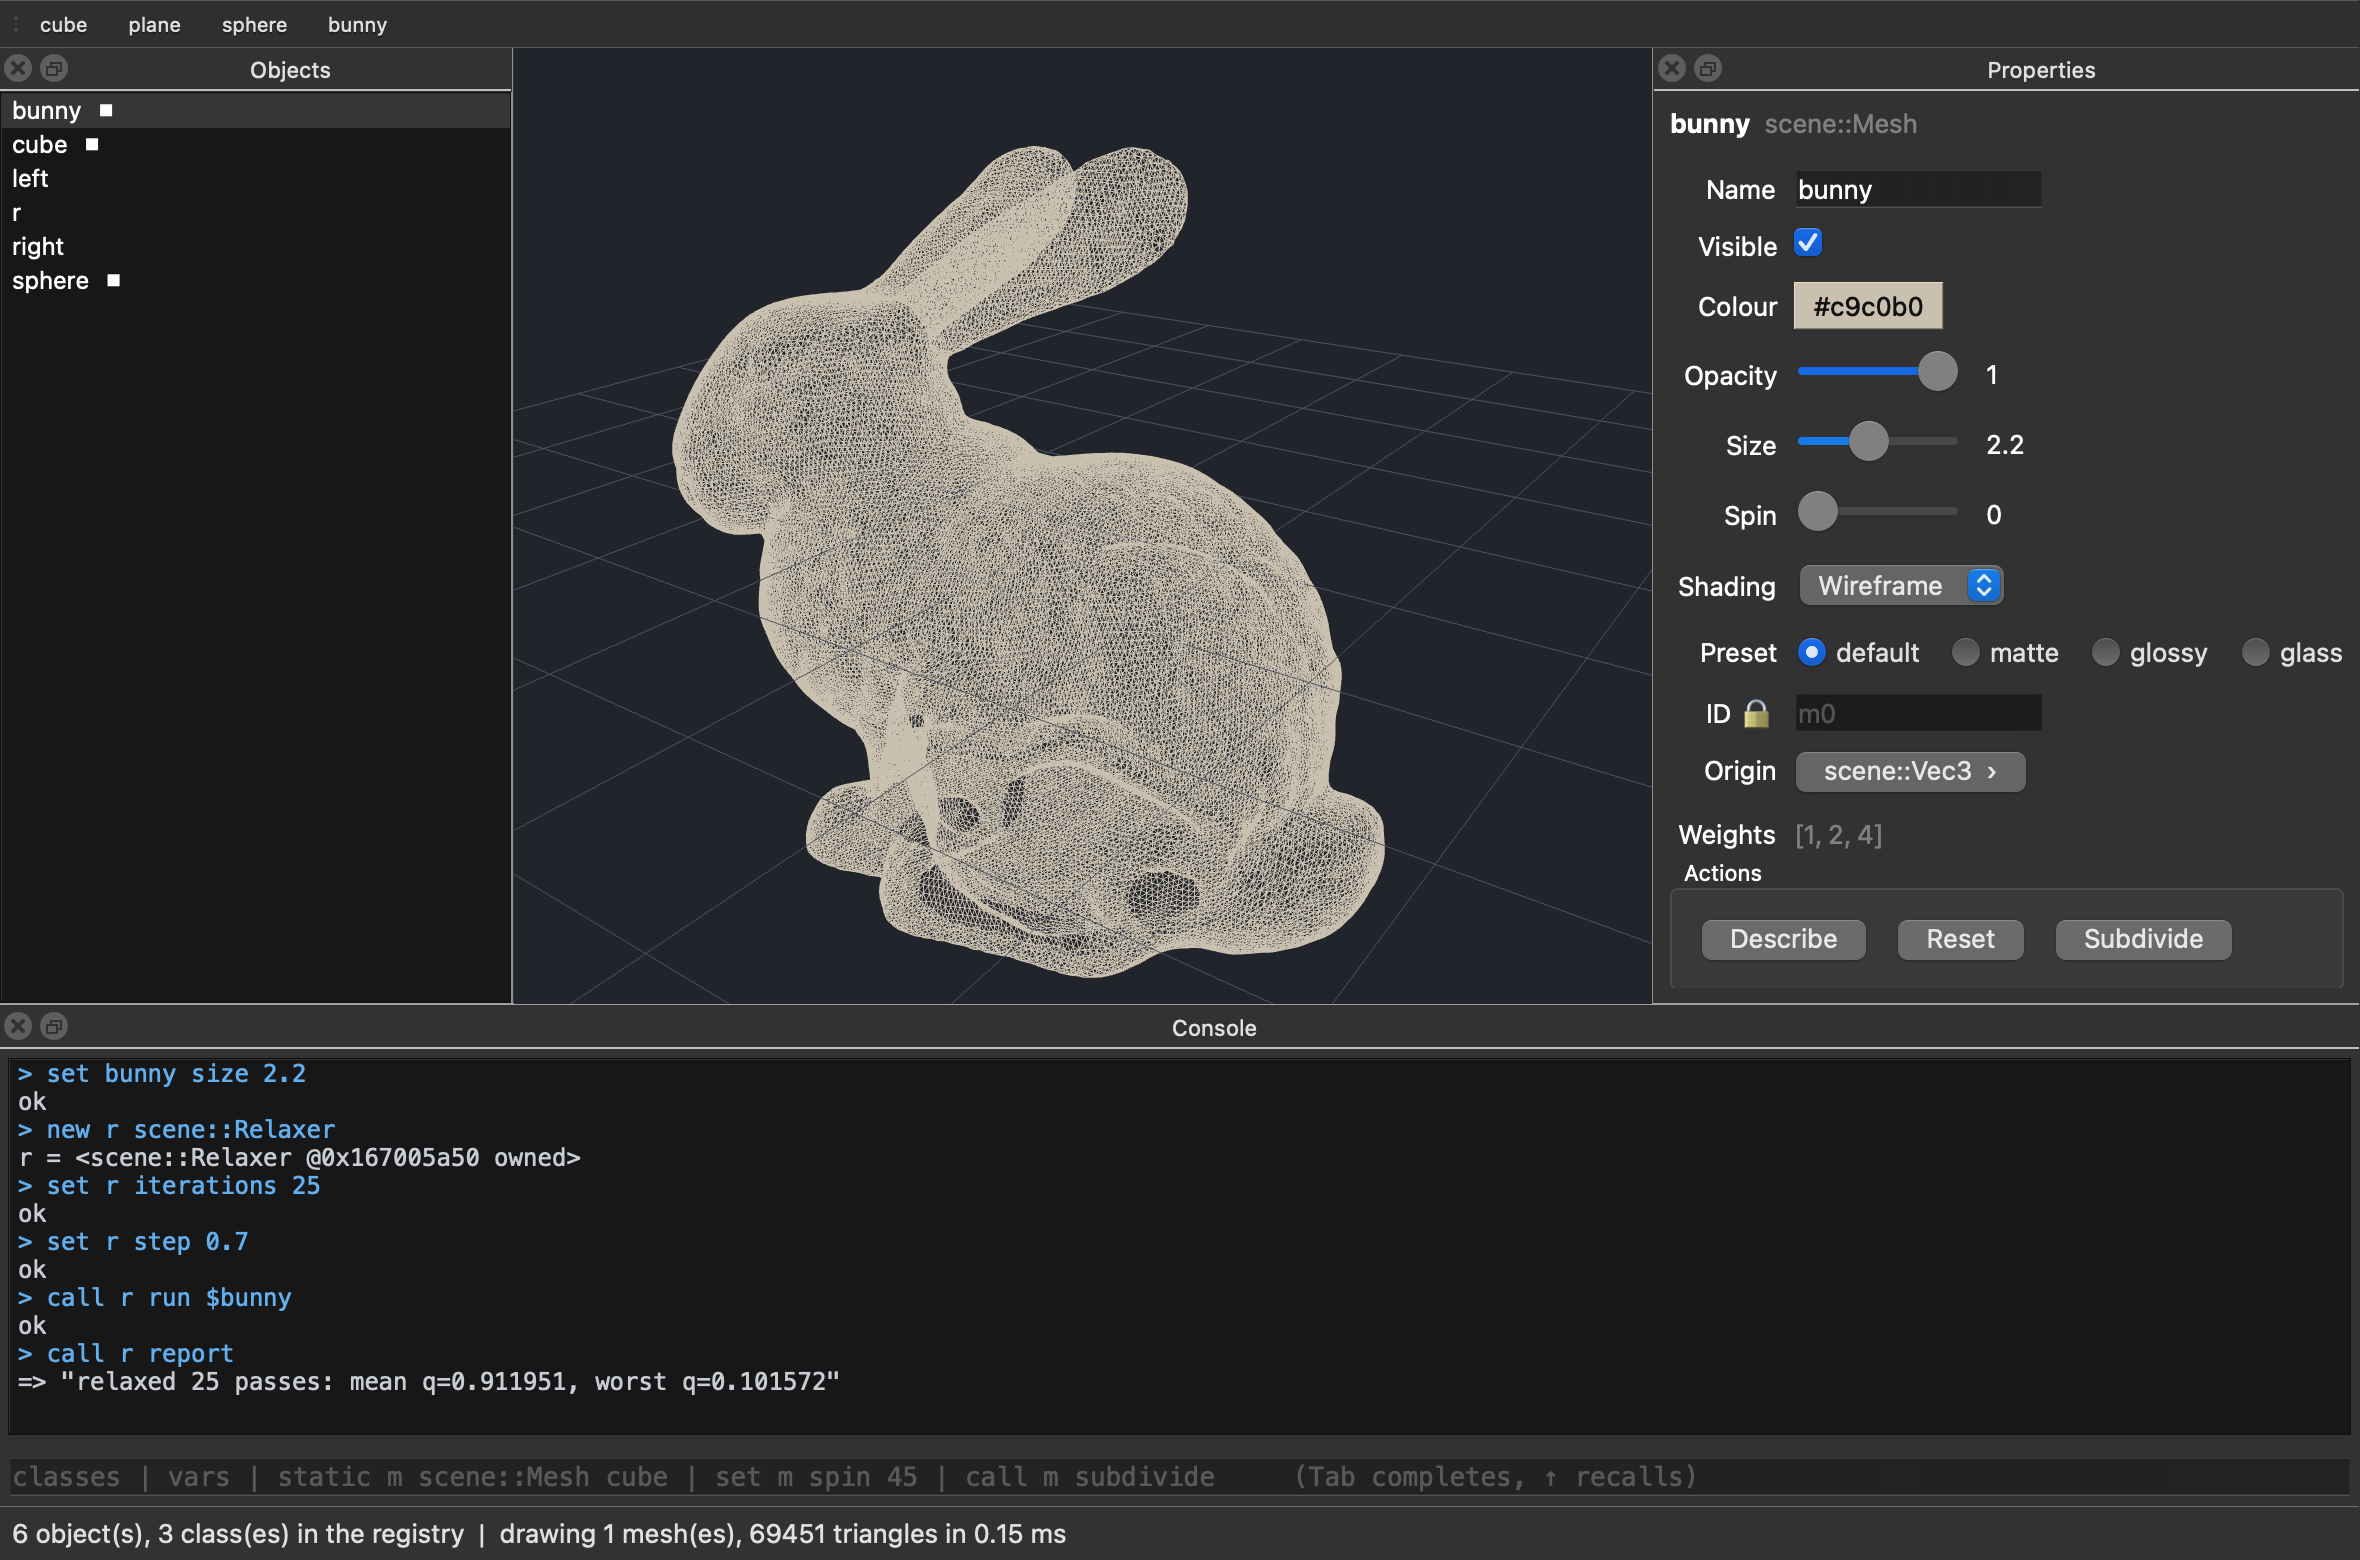
\includegraphics[width=\textwidth]{../figures/e6-viewer.png}
\caption{Le visualiseur Qt après que la bibliothèque a gagné un solveur. La
session console crée un \code{scene::Relaxer}, règle ses paramètres et appelle
\code{run} sur le lapin ; la liste d'objets gagne \code{r} ; la vue se redessine
à partir du maillage muté. Rien dans \code{qt/} n'a été recompilé contre le
solveur, et rien n'y en fait mention --- la fenêtre est construite en
interrogeant des métadonnées qui ont grandi. La feuille de propriétés de droite
est engendrée de la même façon : ses lignes, leurs widgets et leurs bornes
proviennent tous d'annotations voyageant avec les métadonnées plutôt que de code
dans \code{qt/} --- y compris la ligne \code{Preset}, dont les quatre choix sont
lus depuis une annotation \code{combobox} que la vue ne code jamais en dur.}
\label{fig:e6}
\end{figure}

\subsection{La prétention, vérifiée plutôt qu'affirmée}

Une étude de cas peut affirmer n'importe quoi ; celle-ci est donc aussi un test
(\code{E6-case-study/}). La même bibliothèque traverse la chaîne deux fois, la
seule différence étant que le manifeste liste ou non \code{Relaxer}, et les
artefacts engendrés sont comparés. La prédiction est délibérément à deux faces,
car un test d'identité octet pour octet invite à une réussite vide de sens :

\begin{itemize}\setlength{\itemsep}{1pt}
  \item les \emph{métadonnées} doivent différer --- 4 fichiers de l'étape~1
        changent, et \code{Relaxer} est présent dans les tables \og après \fg{} et
        absent des tables \og avant \fg{} ;
  \item la \emph{liaison} ne doit pas changer --- et 0 fichier sur 18 de
        l'étape~2 change, sur 4\,173 lignes engendrées.
\end{itemize}

Les deux se vérifient. Ce second nombre est le propos de la
section~\ref{sec:dynamic} énoncé sous forme d'artefact : la liaison qu'importe un
hôte est une liaison de l'API de réflexion, de sorte que la bibliothèque a grandi
et que la chose dont dépendent tous les consommateurs n'a pas bougé d'un octet.
E2 mesure la même propriété comme un compte de fichiers sur une croissance de
$13\times$ ; ceci la mesure comme une identité octet pour octet sur un changement
concret à l'échelle humaine, et fait échouer l'exécution si cela cesse un jour
d'être vrai.

\paragraph{Ce que cela ne montre pas.} Le banc d'essai compare des artefacts
engendrés ; que les consommateurs écrits à la main fonctionnent encore repose sur
les traces du contrôle de versions ci-dessus, ce qui est plus faible. La
bibliothèque est la nôtre --- une bibliothèque de démonstration assez petite pour
qu'un lecteur la tienne en tête --- de sorte que les preuves sur code tiers
restent à la section~\ref{sec:e5}. Et le plan de cette section promettait
autrefois un bras Julia : la projection \emph{scriptable} livre des convertisseurs
de valeurs pour Python, Lua, Node et WebAssembly, mais pas pour Julia ; ce bras
n'existe donc pas et n'est pas revendiqué.

% =====================================================================
\section{Limites}
\label{sec:limitations}

\begin{enumerate}
  \item \textbf{Chaîne d'outils de recherche.} L'étape~1 exige
    \code{clang-p2996}. Les étapes~0 et 2--3 non, de sorte que les artefacts émis
    survivent au fork --- mais un projet ne peut pas régénérer sans lui.
  \item \textbf{Deux cibles ne sont pas exemptes de réflexion.} L'affirmation de
    la section~\ref{sec:pipeline} vaut pour dix-sept des dix-neuf moteurs. Les
    moteurs \code{rest} et \code{json} émettent des projets dont les sources
    incluent un \emph{visiteur d'exécution} qui insère encore des réflexions au
    moment où la liaison est compilée, et leur \code{CMakeLists.txt} engendré
    demande donc C++26. C'est un choix de conception et non un oubli ---
    réfléchir au moment de la compilation de la liaison garde ces deux émetteurs
    très petits, car le code par membre est écrit une fois sous forme de patron
    au lieu d'être déployé par le générateur --- mais c'est un vrai troc de
    simplicité de déploiement contre simplicité de génération, et cela signifie
    que ces deux cibles héritent de la dépendance au fork. La distinction mérite
    d'être nommée : un moteur peut dépenser la RI soit au moment de la
    génération, soit au moment de la compilation de la liaison, et seul le
    premier cas donne un artefact exempt de réflexion.
  \item \textbf{Les annotations en ligne font perdre la propriété d'exemption de
    réflexion.} Une annotation écrite dans un en-tête utilisateur y attire
    \code{<experimental/meta>}, si bien que la passe appelante a elle aussi
    besoin de C++26. Les annotations hors ligne existent précisément pour éviter
    cela ; elles sont porteuses, non cosmétiques.
  \item \textbf{Les convertisseurs de types sont écrits à la main.} Lire une
    valeur du langage hôte est irréductiblement propre à chaque langage :
    environ neuf méthodes par langage, plus la moitié qui lit.
  \item \textbf{La projection scriptable n'est pas en $O(1)$ de bout en bout.}
    Seule la liaison est indépendante de la bibliothèque : les tables de
    métadonnées sont toujours régénérées à chaque changement, croissant de 95 LDC
    par classe, et le bras scriptable émet \emph{plus} de code au total que le
    bras statique à toutes les tailles mesurées (section~\ref{sec:e2}). Ce qui
    est constant, c'est la liaison, son manifeste et son temps de génération ---
    pas la chaîne.
  \item \textbf{La répartition dynamique a un coût réel.} Recherche linéaire par
    nom et notation des surcharges à chaque accès. Inadaptée aux boucles
    internes ; une poignée de méthode résolue est stable pour la durée du
    processus et peut être mise en cache.
  \item \textbf{Un type vestigial dans chaque module.} La liabilité est décidée
    au moment de la génération et ne peut pas savoir qu'un convertisseur de type
    existera plus tard ; le type de valeur emboîtée doit donc rester dans la
    liste des classes liées, alors même que rien ne le produit jamais
    directement. Un type inutilisé par module.
  \item \textbf{La couverture mesure l'exposition, non la correction.} Une
    méthode liée peut rester fausse ; \code{coverage.json} compte ce qui a
    franchi la frontière, non son comportement.
  \item \textbf{Pas de sémantique formelle.} La RI est définie par son
    implémentation.
\end{enumerate}

% =====================================================================
\section{Travaux apparentés}
\label{sec:related}

\gap{Rédiger la prose autour du tableau~\ref{tab:related} ; citations à compléter.}

\begin{table}[h]
\centering\footnotesize
\begin{tabular}{lccccc}
\toprule
système & découverte des types & intrusion en-tête & cibles & modèle d'exécution & couverture \\
\midrule
SWIG~\cite{swig}            & analyseur propre    & fichier \code{.i} & nombreuses & non & non \\
pybind11~\cite{pybind11}    & écrite à la main    & aucune & 1 & non & --- \\
nanobind~\cite{nanobind}    & écrite à la main    & aucune & 1 & non & --- \\
Qt moc~\cite{qt}            & analyseur propre    & \code{Q\_OBJECT} & 1 & \textbf{oui} & non \\
Graphite/GOM~\cite{graphite}& enregistrement manuel & macros & Lua $+$ IHM & \textbf{oui} & non \\
Unreal UHT~\cite{unreal}    & analyseur propre    & \code{UCLASS} & Blueprint & \textbf{oui} & non \\
cppyy~\cite{cppyy}          & JIT Clang           & aucune & 1 & oui & non \\
générateurs sur AST Clang   & AST Clang           & aucune & 1--2 & non & partielle \\
\midrule
\textbf{\rosetta}           & \textbf{native au langage} & \textbf{aucune} & \textbf{19} & \textbf{oui} & \textbf{oui} \\
\bottomrule
\end{tabular}
\caption{Positionnement. Deux colonnes portent l'écart --- une découverte native
au langage sans intrusion dans les en-têtes, et les deux projections issues d'une
seule description. Tous les systèmes antérieurs en possèdent au plus une.}
\label{tab:related}
\end{table}

L'antériorité la plus proche n'est pas un autre générateur de liaisons mais les
systèmes méta-objet : celui de Qt, le GOM de Graphite et celui d'Unreal. Chacun a
démontré, bien avant C++26, qu'un modèle objet d'exécution peut piloter le
scriptage et des interfaces utilisateur engendrées, et la projection dynamique de
\rosetta{} est explicitement une descendante de cette idée. Ce que chacun exige,
c'est une \emph{description séparée} : un vocabulaire de macros dans l'en-tête
et un analyseur sur mesure, ou bien des appels d'enregistrement manuels. La
contribution de \rosetta{} face à cette lignée est que la description est le
source C++ lui-même, lu par le compilateur, sur des en-têtes qui n'exigent aucune
modification --- et que la même description produit simultanément les liaisons
statiques, ce que les systèmes méta-objet ne tentent pas.

Face à la lignée des générateurs de liaisons --- SWIG, pybind11, nanobind,
générateurs sur AST Clang --- l'écart est inverse. Ces systèmes produisent de
bonnes liaisons pour une ou deux cibles, mais chacun porte soit une façade C++
qui doit suivre l'évolution du langage, soit une spécification écrite à la main
classe par classe, et aucun ne produit de modèle objet d'exécution. \rosetta{} ne
prétend pas à de meilleures liaisons Python que pybind11 ou nanobind ; il prétend
qu'atteindre la dix-neuvième cible ne devrait pas coûter dix-neuf fois la
première.

% =====================================================================
\section{Conclusion}
\label{sec:conclusion}

\gap{À écrire en dernier.}

\todo{Reprendre : la réflexion comme mécanisme de description d'interfaces ; une
RI, deux projections ; le moment de la résolution comme axe expliquant leur
différence ; la couverture comme propriété mesurable d'une interface. Terminer
sur l'étude de cas.}

% =====================================================================
\section*{Disponibilité}
\rosetta{} est disponible à l'adresse
\url{https://github.com/rosetta-bindings/rosetta} sous licence MIT.
\todo{archiver un DOI de version (Zenodo) avant soumission}

% =====================================================================
\bibliographystyle{plain}
\bibliography{../rosetta}

\end{document}
